\documentclass{scutmaster}

\usepackage{pgf}
\usepackage{import}
\usepackage{graphicx}
\usepackage{booktabs}
\usepackage{multirow}
\usepackage{siunitx}
\usepackage{xcolor}
\usepackage{subcaption}
\usepackage[author={胡玮文}]{pdfcomment}
\usepackage{tikz}
\usepackage{wrapfig}
\usetikzlibrary{backgrounds,intersections,calc,positioning,fit,shapes.geometric}
\usepackage{hyperref}

\DeclareMathOperator*{\argmax}{arg\,max}
\DeclareMathOperator*{\argmin}{arg\,min}
\DeclareMathOperator{\sg}{sg}

\newcommand{\TODO}[1]{\textcolor{red}{TODO: #1}\GenericWarning{}{LaTeX Warning: TODO: #1}}

\title{高精度3D人脸重建关键环境\texorpdfstring{\hspace*{\fill}\\\hspace*{\fill}}{}及可微分渲染技术研究}
\titleEN{Research on Key Environment and Differentiable Rendering for High-Precision 3D Face Reconstruction}
\date{\zhtoday}
\dateofsubmit{2023}{4}{19}
\classificationnumber{TP391.41}
% https://www.arocmag.com/html/requirement/201405166.html

\author{胡玮文}
\authorEN{Hu Weiwen}
\studentnumber{202021045611}
\phone{17701952145}
\email{huww98@163.com}
\address{江西省南昌市青山湖区江大南路139号荣昌小区16栋(330029)}

\degree{电子信息硕士(软件工程)}{电子信息硕士}
\major{软件工程}{数字人}

\supervisor{杜卿}{副教授}
\supervisorEN{Assoc. Prof.}{Du Qing}
\supervisorEx{赵巍}

\school{软件学院}

\defensedate{2023年6月3日}
\defensecommittee{王振宇}{汤德佑、向毅、程兴国、袁锋}

\input{build/git_description}
\hypersetup{
    bookmarksnumbered,
    pdfinfo={
        Version=\gitdescription
    }
}

\usepackage{xunicode-addon}
\xeCJKDeclareCharClass{Default}{%
  "24EA,        % ⓪
  "2460->"2473, % ①–⑳
  "3251->"32BF, % ㉑–㊿
}
% 将中文字体声明为(西文)字体族
\newfontfamily\EnclosedNumbers{Noto Sans CJK SC}

% 放置钩子,只让带圈字符才需更换字体
\AtBeginUTFCommand[\textcircled]{\begingroup\EnclosedNumbers}
\AtEndUTFCommand[\textcircled]{\endgroup}

\begin{document}

\maketitle
\hideinblind{
    \maketitleEN
    \nominationpage
    \declareoforiginality
}

\frontmatter
\chapter{摘\texorpdfstring{\quad}{}要}

3D人脸重建方法旨在从照片等现实采集的数据中恢复人脸的3D模型,
这些方法在计算机视觉、图形学和虚拟现实等领域都有广泛的应用。
高精度的人脸重建方法可为影视、游戏等高逼真渲染提供基础,
但其所需数据采集通常需要专业的摄影设备和专门搭建的环境,成本高且实施困难。
基于少量非受限环境照片的重建方法则较为便利,
已被应用于人脸识别、人脸表情捕捉、人脸跟踪、人脸动画合成等任务中。
然而,现有方法未能充分利用照片中的边缘信息,它们依赖2D人脸关键点识别、多目立体等方法以重建人脸的几何形状,这增加了额外的复杂性和累积误差。

为解决高精度人脸数据采集环境要求高,实施困难的问题,
本文提出了一套多视角高精度人脸数据采集方案。
为控制实施难度,该方案尽量利用市面上可购买的部件,
仅包含了少量易于制作的定制硬件。
该方案搭建了完全受控的数据处理管线,
为3D重建所需的采集、标定、数据整理等环节提供了全面的支持,
力求实现高精度、高效率、且灵活可扩展的数据采集,
为基于物理的高精度重建算法提供了坚实基础。

为解决非受限环境照片中边缘信息难以利用的问题,
本文提出了一种基于可微分渲染的3D人脸重建算法。
本文从理论上分析了无法对背景准确建模时的可见性梯度计算问题,
提出了一种面积归一化的像素损失函数。
然后本文进一步分析了该损失函数的作用机理,并与现有可见性梯度计算方法相结合,高效实现了该损失函数。

上述方案已能利用可见性梯度,
然而,人脸只是整个人体模型的一部分,当人脸模型被裁剪下来用于重建时,在人工裁剪的模型边缘会产生异常梯度。
为解决该问题,
本文进一步提出了一种基于SDF贴图的方法对所有渲染图像中的边缘进行分类,从而消除这些异常梯度。
最终使人脸3D模型能合理保持原有拓扑结构,从而提高了重建的准确性和实用性。

基于本文提出的这些方法,本文实现了一个基于逆渲染的完整自动化人脸重建流程。
该流程利用现有神经网络方法进行初始化,并结合传统方法重建人脸纹理。
其重建的人脸可在一定的视角、光照、表情变化下较为逼真的重新渲染。
本文展示和评估了其重建效果。

\keyword{关键词:} 人脸重建;人脸扫描;可微分渲染;逆渲染;SDF贴图

\chapter{Abstract}

Face reconstruction methods aim to recover 3D models of faces from real-world data, such as photos.
These methods have widespread applications in areas including computer vision, graphics, and virtual reality.
High-precision face reconstruction methods provide the foundation for high-fidelity rendering in industries such as film and gaming.
However, the data required for such methods often requires specialized photography equipment and a dedicated setup,
which can be costly and challenging to implement.
Methods based on a limited number of unconstrained photos are more convenient and
have been applied to tasks such as face recognition, facial expression capturing, face tracking, face animation synthesis, etc.,
However, existing methods have not fully utilized the edge information in photos,
instead relying on 2D face landmark detection, multi-view stereo, etc.\ to reconstruct the geometric shape of the face,
which introduces additional complexity and cumulative error.

To address the challenge of high-precision face data collection,
where the requirements for the environment are high and the implementation is difficult,
this thesis presents a scheme for collecting multi-view high-precision face data
that utilizes readily available market components and a few simple DIY hardware for ease of implementation.
This scheme establishes a fully controlled data processing pipeline,
supporting all the requirements of 3D reconstruction, such as data collection, calibration, collation, etc.
The scheme aims to achieve high-precision and high-efficiency, flexibility and scalability.
The collected data provides a solid foundation for physically based high-precision reconstruction algorithms.

To address the challenge of leveraging edge information in unconstrained photos,
this thesis proposes a 3D face reconstruction algorithm based on differentiable rendering.
This thesis analyzes the difficulty  of computing visibility gradients in situations where the background cannot be accurately modeled,
and proposes an area-normalized pixel loss function.
This thesis analyzes the mechanism of this loss function,
and integrate it with the existing methods for computing visibility gradients in general differentiable rendering,
achieving an efficient implementation.

The above method can already utilize visibility gradients.
However, the face model is only part of the whole human model.
When the face model is cropped for reconstruction,
the artificial cut edges can produce abnormal gradients.
To overcome this issue, this thesis further proposes a method based on SDF maps to classify all edges in the rendered images,
which eliminates these abnormal gradients.
By ensuring that the reconstructed face model can reasonably preserves its original topology,
the proposed method enhances the accuracy and practicality of the reconstruction.

Based on the proposed methods, This thesis presents a fully automatic face reconstruction pipeline based on inverse rendering.
The pipeline employs existing neural network methods for initialization and integrates traditional methods to reconstruct the face texture.
The resulting reconstructed face can be realistically re-rendered under certain views, lighting, and expression changes.
This thesis presents and evaluates the reconstruction results.

\keyword{Keywords:} face reconstruction; face scanning; differentiable rendering; inverse rendering; SDF maps

\tableofcontents

\listoffigures

\listoftables

\mainmatter
\chapter{绪论}
\label{chap:intro}

\section{研究背景}

\section{本文研究内容及贡献}

\section{本文组织结构}

本文正文共分为六个章节,各章节的主要内容如下:

\newcommand*{\chapref}[1]{\hyperref[{#1}]{第\ref*{#1}章~\nameref*{#1}}}

\chapref{chap:intro}。
本章介绍了3D人脸重建、以及可微分渲染的背景、关联及意义,
并总结了本文主要贡献及各章节的内容安排。

\chapref{chap:related_work}。
本章对3D人脸重建、可微分渲染相关方向的研究和实践进行了综述,
其中包括\TODO{}。
此外,还介绍了一些可用于3D人脸渲染的计算机图形学的基础知识。

\chapref{chap:method}。
本章介绍了本文提出的一种对现有可微分渲染的改进方法。
该方法能增强可微分渲染技术在难以建模背景的图像拟合任务中的适应能力。
其理论构建在修改的损失函数之上,并通过收缩、扩张两项梯度项来实现。
本章也通过实验验证了该方法的有效性。

\chapref{chap:recon}。
利用上一章提出的方法,本章介绍了一个从单张自然环境照片重建3D人脸的实现。
同时该实现有机结合了神经网络、可微分渲染和一些传统算法,
达成了快速高效,细节丰富且全自动的3D人脸模型重建。
本章也与其他相关工作进行了比较。

\chapref{chap:platform}。
为了更专业地采集基于物理的人脸渲染所需的材质数据,实现更高精度,更逼真的3D人脸渲染效果,
本章介绍了一个多视角人脸重建实验平台。
该平台能够实现高分辨率人脸照片的便捷多视角采集,
并为后续的数据收集整理,相机、光源标定等重建所必备的步骤提供了软件支持。
本章将介绍该平台的软硬件设计思路、实现细节、使用方法以及其可行性初步验证的结果。

\chapref{chap:conclusion}。
基于本文完成的工作结果对本文研究进行总结,并分析当前工作存在的不足和对未来工作的展望。


\chapter{相关研究综述}
\label{chap:related_work}

\section{多视角3D重建}

\section{高效3D人脸重建}

\section{可微分渲染}

\section{高质量人脸3D渲染}

\paragraph{基于物理的渲染}

\paragraph{分离求和近似}

\paragraph{次表面散射}


\chapter{多视角人脸数据采集方案设计与实现}
\label{chap:platform}

若要解决从单张图像同时重建人脸3D模型的几何和材质细节这一高度非适定的问题,则需要更多有关人脸的先验知识。
为此则需要大量高精度的人脸3D几何和材质数据。
这些数据有时候以启发式的算法从2D图像中生成,
但更加鲁棒和贴近物理的方法自然是使用高精度的设备直接采集获得。

然而,可用于实现人脸几何和材质细节高精度重建的解决方案通常价格高昂,其采集的数据往往也由于商业价值较高而不被公开。
因此,不论是采集高精度的数据以重建高精度模型直接用于下游任务,还是用于建立先验以实现更高效的3D人脸重建,都离不开一套精准、高效、可靠的采集方案。

本章提出了一套在较为有限的经济和时间成本下实现的多视角人脸数据采集方案。
该方案除了成本较商业方案显著更低外,
其在设计时考虑到后续研究工作所需的灵活性和可扩展性,并尽量使用可在市面上购买的部件,以减少对硬件相关专业知识的需求。
同时配合一些定制的软件和硬件,实现对各个部件的高效统筹控制,为高精度重建所需的数据采集、标定全流程提供支持。

\section{总体目标}

在功能上,本采集方案的目标是提供基于物理的多视角3D重建算法所需的所有数据,
包括相机拍摄的图像,相机和环境光照的标定数据。
这些数据应尽可能准确地在计算机中还原整个采集过程中相机成像的物理过程。
为实现该目标,本方案包括以下几个部分:
\begin{enumerate}
\item 用于固定相机、灯光的机械结构。需要结构稳固,且能容纳足够数量的设备。
\item 相机、灯光的控制设备。能在精确的时间点触发相机快门和闪光灯闪光。
\item 用于照片拷贝、整理的软件。由于相机数量多,需要专门的方案以提升操作效率,并对接后续标定等算法流程。
\item 相机内外参标定方案。用于准确获取相机焦距等内参以及相对位置等外参。
\item 环境光照标定的方案。可用于基于物理光线传播模型估计人脸材质。
\item 采集过程中人工操作的标准操作流程。用以保证采集数据的质量。
\end{enumerate}
本文在设计该采集方案时,除了以上功能性目标外,还主要考虑了以下非功能性目标:
\begin{itemize}
\item 低硬件专业技能需求。本项目作为软件学院个人参与的项目,其所能得到的机械、结构、电子等方面的专业技术支持非常有限。
因此,为了能在有限的时间内完成该项目,本文尽可能地使用市面上可购买的部件,以减少对相关专业知识的需求。
虽然如此,本文还是使用了少量定制的硬件。

\item 高精度。高精度的数据是高精度3D重建的基础。
因此,对误差的控制贯穿于采集流程的各个环节,指导整个采集方案的软硬件设计。

\item 高效。整个系统在使用时,特别是在对被拍摄对象拍照时,应该尽可能地快速,使大规模数据收集成为可能。

\item 灵活。本方案作为一个主要用于研究性工作的采集系统,其需要具有一定的灵活性,以便应对研究中多变的需求。
基本地,该系统应能同时支持被动光源和主动光源的采集,能灵活配置相机和光源的位置和其他相关参数。

\item 可扩展。即使在本文写作完成后,该系统仍很可能被继续用于后续的研究工作。因此本方案也应适当考虑未来可能的更大规模的采集需求。

\end{itemize}

利用本方案采集的数据预计可用于多种3D人脸重建算法,例如本文其他部分介绍的基于可微分渲染的逆渲染方法。
同时也可用于如多目立体等传统的计算机视觉算法。

本章的主要贡献在于对该方案各个部分的设计和实现,以及对其性能的评估验证。
本章的剩余内容将具体介绍该方案的各个部分。

\section{方案设计}

\subsection{支撑机械结构设计}

\begin{tikzpicture}[
    every node/.style={anchor=north west, minimum height=0.8cm},
]
\node [draw, minimum width=6cm] (A) at (0,0) {相机支架底座};
\node [draw, minimum width=2.4cm] (layer1) at (0,1) {高度层};
\node [draw, minimum width=2.4cm, right=0 of layer1] (layer2) {高度层};
\node [draw, minimum width=1.2cm] (camera1) at (0,2) {相机};
\node [draw, minimum width=1.2cm, right=0 of camera1] (camera2) {相机};
\node [draw, minimum width=1.2cm, right=0 of camera2] (camera3) {相机};
\node [draw, minimum width=1.2cm, right=0 of camera3] (camera4) {相机};
\node [draw, minimum width=1.2cm, base right=0 of layer2, minimum height=1.8cm] (camera5) {相机};
\node [draw, right=of A] (B) {灯架};
\end{tikzpicture}

本方案的硬件框架结构设计主要是参考了\citet{RiviereGBGB20}所展示的布局。
首批配置了12台相机和4台带有柔光箱的摄影灯,其中相机固定在3个铝型材搭建的、定制的、高自由度可调节的支架上。
灯则由于其体积质量较大,且市面上缺少相应的单独连接件产品,无法稳固地固定在支架上,因此直接使用了单独的专用灯架固定,以确保安全。
图\ref{fig:HDRI}展示了该系统硬件的整体布局。

\begin{figure}
\centering
\begin{subfigure}[b]{0.3\textwidth}
    \centering
    \includegraphics[height=7cm]{figures/frame-design}
    \caption{设计图}
\end{subfigure}
\begin{subfigure}[b]{0.2\textwidth}
    \centering
    \includegraphics[height=7cm]{figures/frame-impl}
    \caption{组装完成照片}
\end{subfigure}
\begin{subfigure}[b]{0.47\textwidth}
    \centering
    \includegraphics[height=7cm]{figures/frame-camera}
    \caption{相机固定}
\end{subfigure}
\caption{铝型材支架的设计和实现}
\label{fig:frame}
\end{figure}

图\ref{fig:frame}展示了铝型材支架的设计和实现。
单个支架的主体部分由4个2寸脚轮,12.47米3030铝型材以及若干连接件组成。
设计全高2.103米,长1.06米,宽0.53米。
其物料成本约需要700元。
考虑到实验场地可能的变动,支架装配有4个脚轮,方便移动,且这些脚轮带有锁定功能,在使用时也能固定支架的位置。
脚轮固定在矩形底座上,底座则通过大量连接件,尽可能稳固地支撑了两根2米长的竖直铝型材。
在竖杆之间设计有4根长1米的横杆。
每两根间设计间距为0.5米,但得益于本方案使用T型螺母固定,无需打孔,因此这些横杆的位置可根据需要随时调整。

相机可固定在任意竖杆和横杆上的任意位置。
为固定相机,本方案首先将T型连接板通过T型螺母固定在铝型材上,然后将一个球形云台通过1/4英寸螺栓固定在连接板上,最后将相机通过标准的1/4英寸接口固定在云台上。
使用云台可允许相机以三个自由度任意旋转,再加上相机固定位置,横杆位置,以及支架整体的移动,相机最终固定位置的可调节自由度非常高。

总的来说,该支架支撑稳定,使用灵活,完全满足了固定12台相机的需求,为其他部分的实现打下了良好的基础。
同时,通过增加横杆,或增加支架数量的方式,也可以扩展更多相机固定位置。

\subsection{被动相机同步}
\label{sec:passive_sync}

本方案使用的是CVTE提供的12台消费级微单相机,型号为佳能R6。
将这些相机固定在支架上后,下一步就需要对它们集中进行控制。
其中最简单的形式就是使它们精确地在同一时刻触发快门,以确保后期重建过程不会受到被拍摄对象的位移或形变影响。
为此,本方案中设计了一种用于相机同步的硬件装置。
该装置构造简单,且无须独立供电。它能以很高的时间精度同时触发多台相机的对焦和快门,从而实现人脸多视角数据的捕获。

\paragraph{相机快门触发原理}

为设计该装置,本文首先调查了所使用的相机所有可能的快门触发方式,包括:
\begin{itemize}
\item 相机机身上的快门按钮。该按钮半按可触发对焦,全按可触发快门。
然而使用机械方式触发快门对自动化控制系统来说显然过于复杂,且容易造成不必要的机械震动。
\item 网络接口。该相机支持连接Wi-Fi或蓝牙,并可通过佳能的私有协议或者基于HTTP的Camera Control API控制。
但是无线网络连接会引入毫秒级别的不确定性延迟,因此不适合用于本方案中高精度的同步控制。
\item 快门线接口。该相机支持通过2.5mm快门线接口触发快门,该接口仅需要简单地控制电路通断即可触发对焦和快门。
\item USB连接。该相机支持通过USB连接上游设备,且可通过佳能的私有协议控制。
该方案虽然可以实现更多控制功能,且USB还能直接为相机供电,
但相比上一种方案,上游控制设备的开发过于复杂。且佳能官方仅提供了Windows平台的SDK,这更提高了开发难度。
\end{itemize}
基于这些考虑,本方案最终使用了快门线接口作为相机同步的触发方式。

用于快门线接口的2.5mm插头如图\ref{fig:2.5mm}所示。
该插头的接触部分呈旋转对称的柱体,柱体不同高度上分布有3个独立的接触区域,分别对应对焦控制、快门控制和地线。
其中两根控制线待机时为带有上拉的输入端口,电压为3.3v。当其与地线短接,从而拉至低电平时,即可触发对应的控制。
此外,当手动按下相机快门按钮时,这些控制线也会输出低电平,以便于控制其他外设。

\begin{figure}
\centering
\begin{minipage}{.5\textwidth}
    \centering
    \includegraphics[height=3cm]{figures/2.5mm}
    \captionof{figure}{快门线接口的2.5mm插头}
    \label{fig:2.5mm}
\end{minipage}%
\begin{minipage}{.5\textwidth}
    \centering
    \includegraphics[height=5cm]{figures/passive_sync_topo}
    \captionof{figure}{被动同步装置的连接拓扑结构}
    \label{fig:passive_sync_topo}
\end{minipage}%
\end{figure}

\paragraph{被动同步装置设计}
如上所述,若要控制所有相机同时触发快门,则仅需将所有相机的快门控制线连接到同一个按钮上,在按下该按钮时,使所有控制线和地线短接即可。
但其中设计的难点在于,被控制的相机数量较多,有12台且可能在未来进一步扩展,且相机在空间上较为分散。
因此,为了节约线材,并提升操作的便捷性和装置的可扩展性,本方案设计了一种可串联的相机控制器。
控制器与控制器,控制器与相机间的连接拓扑如图\ref{fig:passive_sync_topo}所示。
控制器间可以任意方式连接,构成星型、树形或链式等多种不同拓扑,每个控制器最多能与3个其他控制器以及8台相机相连。
该结构可通过增加控制器的方式近乎无限扩展,从而实现对更多相机的控制。
此外,每个控制器上都是对等的,通过任意一个控制器上的按钮均可控制所有相机。
这提升了系统操作的便捷性。

\begin{figure}
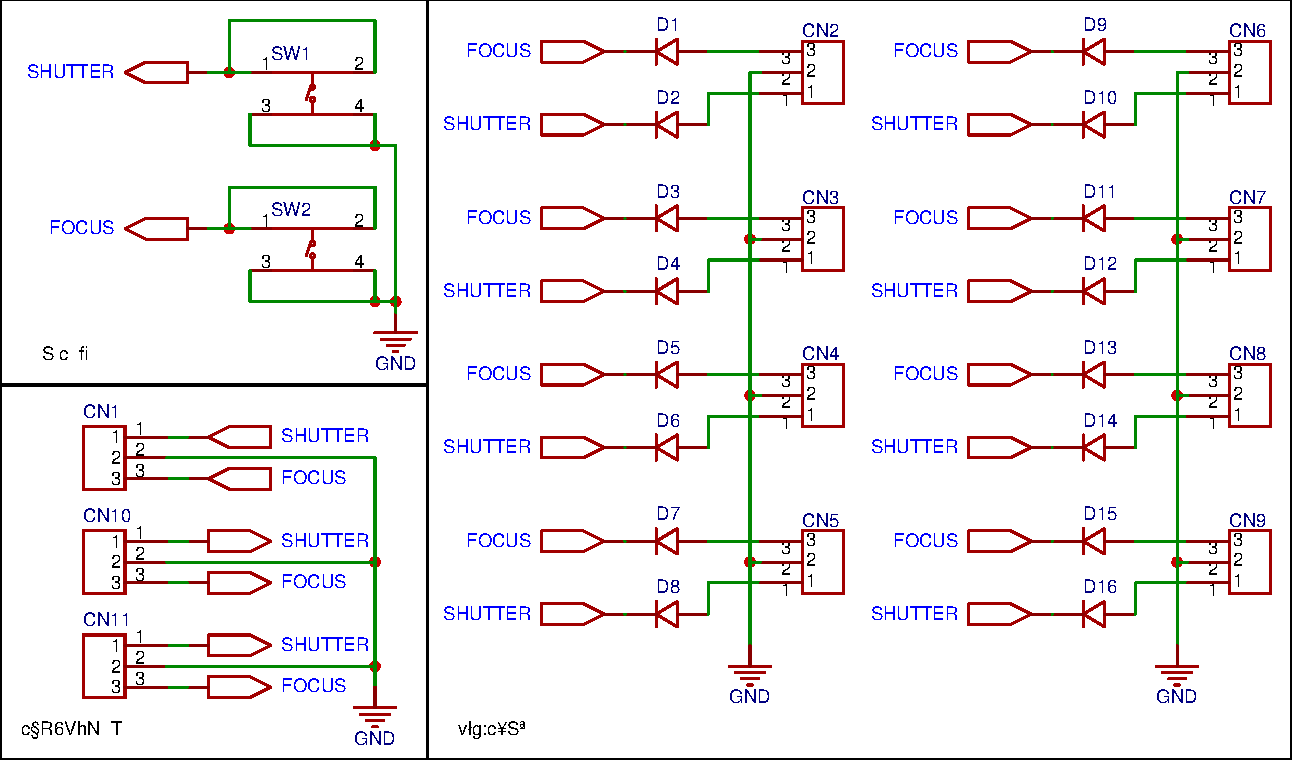
\includegraphics[width=\textwidth]{figures/passive_sync_schematic}
\caption{被动控制器的电路原理图}
\label{fig:passive_sync_schematic}
\end{figure}

\begin{figure}
\centering
\includegraphics[height=5cm]{figures/passive_sync_controller}
\caption{被动控制器的实物图}
\end{figure}

其中,每个控制器的原理图如图\ref{fig:passive_sync_schematic}所示。
控制器无需供电,它采用机械按钮的形式完成控制线和底线的短接,从而触发相机快门。
控制器之间,以及相机与控制器间均采用AWG28规格的排线连接,
在控制器端均使用了冷压的XH2.54插头;
在相机段则使用了焊接的2.5mm插头。
此外,每个相机接口在连接到总线前均使用了两颗二极管进行隔离,以防止相机间的干扰。
这样可允许在控制器连接后依然可以手动控制单台相机的快门,也能防止在连接线缆时误触发快门。

\paragraph{同步精度测试}

\begin{figure}
\centering
\begin{subfigure}[b]{0.55\textwidth}
    \includegraphics[width=\textwidth]{figures/passive_sync_test}
    \caption{测试过程示意图}
\end{subfigure}%
\begin{subfigure}[b]{0.44\textwidth}
    \includegraphics[width=\textwidth]{figures/LED_array}
    \caption{单片机和LED阵列}
\end{subfigure}%
\caption{被动同步装置的同步精度测试装置}
\label{fig:passive_sync_test}
\end{figure}

电场的传播速度非常快,因此,当控制器的按钮被按下时,理论上控制信号能同时送达所有相机。
为了实际测试该装置的效果,本文进行了端到端的同步精度测试。
如图\ref{fig:passive_sync_test}所示,该测试的拍摄目标包括5个由单片机控制的LED灯,以及一个60Hz刷新率的显示器(此处使用iPad)。
其中单片机通过硬件计时器中断精确控制LED灯,每个LED灯的亮灭切换间隔依次为0.5ms、1ms、2ms、4ms、8ms,每16ms这些LED灯的状态完成一次循环。
显示器则显示一个秒表,用于判断16ms以上的时间间隔。

相机摆放时,需要使LED灯在不同相机传感器的同一位置成像,以避免滚动快门的影响。
拍摄前,需要将快门速度调整为最快的1/4000秒,以尽量避免相机曝光过程与LED的亮灭切换过程重叠,影响读取LED灯的状态。
测试时,将两台相机连接在控制器上,然后多次使用控制器触发快门。
读取结果时,首先丢弃难以判断LED灯状态的图像,
对剩余图像以二进制编码的形式记录LED灯的状态以及屏幕显示的秒表的时间。
对比同一次快门中不同相机拍摄到的照片中读数即可准确获得两台相机曝光的时间差,即控制器的同步精度。

实验结果显示,多台佳能R6相机间的同步精度小于0.5ms,即每次拍摄中不同相机的读数均相同。该精度已经足够满足实际应用的需求,且已经远高于快门滚动的速度。
因受到相机最高快门速度的限制,未能以更高的精度完成测试。
此外,本文也测试了R6和另一台佳能90D单反相机间同步的精度,结果显示两台相机间有4ms但非常稳定的延迟。

\subsection{多相机内外参联合标定}
\label{sec:camera_calib}

为了准确建模相机成像的光学过程,建立三维物体与二维照片之间的对应关系,需要对相机的内参和外参进行标定。
即准确测量采集过程中用到的每一台相机的内参和外参。
其中,内参包括相机的焦距、光心坐标、畸变参数等,
外参则包括不同相机之间的相对位置和姿态。

本方案选用的相机模型是针孔相机模型,这也是在实验中采用的相机所遵循的模型。
由于本实验中相机畸变较小,简单起见,本文选用了OpenCV中默认的径向和切向相机畸变模型\citep{opencv_cam}。
更正式地,假设共有$N$个相机,对于第$i$个相机($i=1,2,\cdots,N$),
内参标定的目标是求解该相机的
焦距$f_x^{(i)},f_y^{(i)}$、
光心坐标$c_x^{(i)},c_y^{(i)}$、
畸变参数$k_1^{(i)},k_2^{(i)},k_3^{(i)},p_1^{(i)},p_2^{(i)}$;
外参标定的目标则是求解该相机在世界坐标系下的
位置$\mathbf{t}^{(i)}=\left(x^{(i)},y^{(i)},z^{(i)}\right)$
和姿态$\mathbf{r}^{(i)}$。
其中$\mathbf{r}\in \mathbb{R}^3$为表示三维旋转群$\mathrm{SO(3)}$的的指数映射向量,
其表示轴为$\mathbf{r}$,角度为$\left\| \mathbf{r}\right\|$的旋转。
世界坐标系的选取是任意的,因此在相机标定阶段,不失一般性地,我们选择第一次快门触发时的标定板坐标系为世界坐标系。
\def\camparam{\delta}
综上,在标定过程中共需要求解$N\times 15$个参数,记为$\camparam$。
在该模型下,对于任意在世界坐标系下的点$\mathbf{X}\in \mathbb{R}^3$,其在第$i$个相机的成像平面的投影点$\mathbf{x}^{(i)}$的计算过程可称为相机投影,记为$\mathbf{x}^{(i)}=\pi(\camparam_i, \mathbf{X})$。
$\pi$的形式化定义可参见附录\ref{app:camera_model}。

为了解算上述模型中的参数,通常需要使用待标定的相机对一类特殊的物体进行拍摄,称为标定物体。
它们的特点是通常有一些在照片中容易被计算机视觉算法识别的特征点,且这些点容易在不同相机拍摄的照片间进行匹配。
这类物体通常为标定板,即印有棋盘格、二维码、圆形或者其他易于识别的图案的硬质平面板子。
也有一些方法\cite{colmap}使用SIFT等特征点算法来自动从任意被拍摄物体上提取和匹配特征点。但这种方法匹配成功率稍低,且忽略了物体反射光线的各向异性,因此可能会带来一些误差。

\paragraph{数据采集}
\begin{figure}
    \centering
    \begin{minipage}{0.5\textwidth}
        \centering
        \includegraphics[height=6cm]{figures/april_board}
        \captionof{figure}{April Board上的二维码和棋盘格图案}
        \label{fig:april_board}
    \end{minipage}%
    \begin{minipage}{0.5\textwidth}
        \centering
        \includegraphics[height=6cm]{figures/bayer}
        \captionof{figure}{Bayer格式照片示意图}
        \label{fig:bayer}
    \end{minipage}%
\end{figure}

本方案中使用的标定物体为April Board,即印有二维码和棋盘格组成的图案的标定板,如图\ref{fig:april_board}所示。
该标定板的尺寸为$800 \times 800$毫米,每个二维码的边长为$88$毫米。
该图案中棋盘格的十字角点可由算法精确完成亚像素级定位,而密集的二维码则便于在不同照片中便捷地匹配角点。
其采用了玻璃基板,以保证标定板的刚性和平整度;
同时采用了氧化铝表面,使标定板表面无明显镜面反射光斑,确保标定板在不同光照条件下的可靠性。

在拍摄标定物体时,需要注意保持相机处于手动对焦模式,关闭光学防抖,以防止其内外参意外发生变化。
并使用前述(第\ref{sec:passive_sync}节)被动相机同步装置同时触发所有相机进行拍摄。转动标定板,重复触发快门15-20次。

\paragraph{相机标定优化目标}
\def\cornerpix{\mathbf{o}}
\def\cornerboard{\mathbf{w}}
本方案中的相机标定算法接收照片中的特征点坐标作为输入,求解上述相机模型中的参数$\camparam$。
正式地,假设共触发了$M$次快门,标定板中共有$K=144$个角点,算法的输入包括第$i$个相机在第$j$次触发快门时拍摄的第$k$个角点($j = 1,2,\cdots,M$、$k = 1,2,\cdots,K$)在像素坐标系中的坐标$\cornerpix_{i,j,k}\in \mathbb{R}^2$;
以及角点在标定板坐标系中的坐标$\cornerboard_k\in \mathbb{R}^3$。
由于每次触发快门时标定板都由人工转动,因此其在世界坐标系中的位置也是未知的,故将第$j$次快门时标定板坐标系到世界坐标系的刚体变换$T_{j}(\cdot)\in \mathrm{SE(3)}$也做为未知量。
其中固定$T_{1}$为幺元,即$T_{1}(X) = X$,以确定世界坐标系的位置。
则本文中的相机标定问题可以表示为以下最小二乘优化问题:
\begin{equation}
    \label{eq:calib_opt}
    \argmin_{\camparam,T} \sum_{i,j,k} \left\| \cornerpix_{i,j,k} - \pi\left(\camparam_i, T_j(\cornerboard_k)\right) \right\|_2^2
    \text{。}
\end{equation}
为实现该目标,首先需要在每张照片中识别角点,并以亚像素级精度精确定位其坐标$\cornerpix_{i,j,k}$。
本节后续将介绍角点的识别、精确定位,模型初始化及上述优化问题的具体求解方法。

\paragraph{角点识别}为识别标定板中可供拟合的角点,本文首先识别照片中的二维码,并将二维码的四个角作为角点的候选点。
本文所用标定板上的二维码为AprilTag,本文实现的识别算法也是基于其开源的方法\cite{AprilTag}。
该算法是一个自下而上的算法,它首先从照片中识别直线段,然后将直线段组合成四边形,最后试图将四边形区域识别为二维码。得益于二维码的纠错功能,虽然该方法召回率稍低,但查准率非常高。同时二维码中存储的信息可用于角点在不同照片中的匹配。

本文所实现的版本的输入为相机拍摄的,原始Bayer格式的照片,该照片是单通道图像,其中RGB像素排列如图\ref{fig:bayer}所示,每$2\times 2$个像素中包括一个红色像素、两个绿色像素和一个蓝色像素。每种像素的传感器前带有滤光片,仅允许特定波长的光被传感器捕获。因此,Bayer格式的照片中,每个像素的值即为该像素对应的颜色通道的光照强度。
为了减少冗余的数据处理流程,并保持全流程的可解释性以准确控制误差,本方案直接使用了原始照片,而没有使用常见的相机后处理后输出的RGB格式图像。

由于我们所拍摄的照片分辨率远超二维码识别所需,因此本文先对照片进行降采样。
其具体方法是,首先在每4个像素中仅取一个绿色像素,以排除颜色对二维码识别的影响;
再进行5倍平均池化,即最终降采样后的图像长宽为原图的$1/10$。
以此降低算法耗时并大大降低照片中的噪声等级,提升算法的鲁棒性。
在低分辨率的图像上完成二维码识别后,二维码的四个角的坐标将被重新映射回完整分辨率的像素坐标,以初始化后续的精确定位步骤。

% 本文使用的相机拍摄的原始照片分辨率高,可达$5472\times 3648$;
% 且宽容度高,其量化后的亮度可达约13000级,相比普通JPG照片仅有256级。
% 因此,本文在\cite{AprilTag}的基础上,设计了尺度、亮度无关的直线段识别算法,使其更加鲁棒,并减少算法超参数调节的麻烦。
% \TODO{尺度、亮度无关的直线段识别算法}

\paragraph{角点精确定位}在上一步识别出角点后,该步骤依据角点周围的像素值,获取这些角点尽可能精确的像素坐标$\cornerpix_{i,j,k}$,以保证标定的精度。
该步骤的难点在于,算法需要对失焦造成的模糊、成像过程中的噪声等因素足够鲁棒,并达到亚像素级的精度。
本文采用的算法为\citet{ROCHADE}提出的精确角点定位算法,其基本思想为:
使用一个二维多项式函数对角点周围的像素进行拟合,然后以该多项式函数的鞍点作为该角点的精确像素坐标。

具体地,本文首先需要从照片原始数据获取单通道灰度图。
该灰度图在标定板区域的每个像素值应表征标定板表面反射的总光强,而不与颜色有关。
为此,需要对红色、蓝色像素值进行缩放,使其与绿色像素匹配(相当于相机的白平衡操作),其缩放系数与环境光照、标定板材质等有关。
本文假设标定板任意位置反射的光线的波长分布是均匀的。
因此,本文首先对上一步求得的二维码区域求凸包,以定位照片中的标定板,并调整缩放系数以使该区域中不同颜色像素的均值相等。
然后,对该图使用半径为$r$的圆锥形kernel进行滤波,以使像素值平滑,从而能更好地被多项式函数拟合。
最后,以角点的当前估计位置为中心,使用二阶二维多项式函数对周围的$(2r+1) \times (2r+1)$个像素进行最小二乘拟合:
\begin{equation}
    \label{eq:poly}
    \hat{a} = \argmin_{a} \sum_{x,y} \left(\bar{\mathcal{I}}(x, y) - (a_0 x^2 + a_1 y^2 + a_2 xy + a_3 x + a_4 y + a_5)\right)^2
    \text{,}
\end{equation}
其中,$\bar{\mathcal{I}}$为滤波后的灰度图。
在实现上,本方案直接使用解析公式求解该线性最小二乘问题。并求该二维多项式函数的鞍点作为该角点新的估计位置:
\begin{equation}
    \label{eq:subpixel}
    \begin{cases}
        x' &= -\dfrac{\hat{a}_2 \hat{a}_4 - 2 \hat{a}_1 \hat{a}_3}{\Delta} \\
        y' &= -\dfrac{\hat{a}_2 \hat{a}_3 - 2 \hat{a}_0 \hat{a}_4}{\Delta}
    \end{cases},\quad
    \Delta = 4 \hat{a}_0 \hat{a}_1 - \hat{a}_2^2
    \text{,}
\end{equation}
并如此迭代,直到角点的估计位置收敛,该收敛的位置即为$\cornerpix$。
在此过程中,若估计位置超出了图像范围,或$\Delta < 0$,则将该角点排除。
$\Delta < 0$的原因通常是该角点被其他物体遮挡,或者受到其他物体投下的阴影影响。

\def\cornerincode{\hat{\cornerpix}}
在该算法中,$r$的选取可能对结果产生较大影响。较大的$r$将能利用照片中更多像素的信息,从而对噪声更加鲁棒,但也不能过大,否则周边的二维码,或相邻的其他角点等无关信息将影响拟合结果。为此,本文依据上一步识别到的二维码的尺寸以自适应地选择$r$。令$\cornerincode_{i,j}$为照片中第$i$个二维码的第$j$个角点的估计位置,$j\in\{0,1,2,3\}$,以顺时针方向排列,则$r$的选取为:
\begin{equation}
    \label{eq:r}
    \begin{aligned}
        l_{i,\textrm{edge}} & = \min_j\left(\|\cornerincode_{i,j} - \cornerincode_{i,j+1\bmod 4}\|\right)\text{,} \\
        l_{i,\textrm{diag}} & = \min\left(\|\cornerincode_{i,0} - \cornerincode_{i,2}\|, \|\cornerincode_{i,1} - \cornerincode_{i,3}\|\right)\text{,} \\
        r & = \min_i\left\{0.07 l_{i,\textrm{edge}}, 0.05 l_{i,\textrm{diag}}\right\}\text{。}
    \end{aligned}
\end{equation}

\paragraph{多相机内参标定与外参传递}
获得角点精确位置后,本文分为两个阶段求解公式\eqref{eq:calib_opt}。
在第一阶段,本文将对每台相机分别进行标定,获得各相机的内参初始化值
并估计标定版在每次触发快门时与各台相机的相对位置。
具体地,本文依据相机和镜头厂商提供的传感器尺寸、图像分辨率、镜头焦距初始化相机内参$f$、$c$。
然后调用OpenCV中单台相机标定的算法,使用PnP算法求解标定板在每次触发快门时与相机的相对位置$T_{i,j}$;
并使用Levenberg-Marquardt算法对这些参数进行调整。

由于不同相机的同一次快门的触发是严格同步的,因此可以认为若不同相机在同一次快门的触发时,拍摄到的标定板在世界坐标系中的位置是相同的。
据此可将每台相机,以及每次快门触发作为节点,构建二部图,图中的边表示该相机在该次快门中拍摄到了标定板。
若该二部图是连通图,则可迭代地将所有相机、所有快门触发中的标定板的位置传递到世界坐标系中,
如算法\ref{alg:calib_init}所示。
并最终获得$\delta$和$T$中所有参数的初始化值。

\begin{algorithm}[t]
    \caption{外参传递}
    \label{alg:calib_init}
    \begin{algorithmic}[1]
        \Require 连通二部图$(V,E)$;第$j$次快门时标定版坐标系到相机$i$坐标系的刚体变换$\hat{T}_{i,j}\in SE(3),(i,j)\in E$
        \Procedure{外参传递}{$V,E,\hat{T}_{i,j}$}
            \State $C \gets \emptyset$\Comment{已传递的相机集合}
            \State $T_{1} \gets \mathbf{I}$\Comment{以第$1$次快门时标定版坐标系作为世界坐标系}
            \State $S \gets \{1\}$\Comment{已传递的快门触发集合}

            \While{$C \cup S \neq V$}
                \State $i \gets \forall i\in V| i\notin C, \exists j\in S| (i,j)\in E$
                    \Comment{选择与已知位置的标定板相邻的相机}
                \State $U_{i} \gets T_{j}\hat{T}_{i,j}^{-1}$
                    \Comment{相机$i$到世界坐标系的变换}
                \State $C \gets C \cup \{i\}$
                \ForAll{$j | (i,j)\in E, j\notin S$}
                    \State $T_{j} \gets U_{i}\hat{T}_{i,j}$
                        \Comment{第$j$次快门时标定版到世界坐标系的变换}
                \EndFor
                \State $S \gets S \cup \{j\in V| (i,j)\in E\}$
            \EndWhile
            \State \Return $U, T$
        \EndProcedure
    \end{algorithmic}
\end{algorithm}

\paragraph{集束调整}在第二阶段,本文将对所有相机进行集束调整,即直接使用公式\eqref{eq:calib_opt}中的目标函数,在上一阶段的初始化值的基础上,同时优化模型中的所有参数。
具体地,本文使用了Levenberg-Marquardt算法\cite{lm},对目标函数进行优化求解。
并手动实现了公式\eqref{eq:calib_opt}的雅克比矩阵的解析求解算法,以提升算法的速度和收敛精度。

然后,排除掉误差较大的角点,再次重复上述优化过程,并如此迭代数次,每次使用更严格的误差阈值进行排除。
这些误差较大的角点通常是由于角点定位不准确造成的,因此,将其排除后可以提高标定的精度。
该优化过程最终得到的相机参数$\camparam$即为所求的最终的相机标定结果。


\subsection{基于反射球的光源标定和HDRI合成}
\label{sec:light_calib}

除了相机外,在实验室中拍摄,环境光照信息也可以提前采集,从而获得比用算法从人脸照片中估计更精准的结果。
这些信息可用于后续逆渲染的优化之中。
如前文所述,本装置使用的照明为4盏带有柔光箱的摄影灯,均布置在被拍摄对象正面180°的范围内。光源标定的目的是获取被拍摄对象所处的空间中的每个位置上来自每个方向的光照强度,即光场信息。
但本设备的柔光箱据被拍摄对象约1.5米远,相比来说,人脸的尺度较小,因此,本文假设所有光线均来自无限远,即该光场的分布近似于与空间位置无关而只与光线入射方向有关。

光照强度和方向的对应关系可被编码在一张HDRI(High Dynamic Range Image,高动态范围图像)中,该图像中的每个像素点对应于一个方向,像素点的颜色值则对应于该方向上的光照强度和频率分布。
其与普通的照片保存格式不同,之所以称之高动态范围,是因为其每个像素点的颜色值通常作为浮点数保存,因此可以同时记录很强和很弱的光照,同时保持较高的精度。
使用该技术编码的光照信息也常被用于计算机图形学领域。
如图\ref{fig:HDRI}是一张以本节所述方法合成的,记录了本文目前实验环境的HDRI。
\begin{figure}
\begin{tikzpicture}
    \node [inner sep=0pt, anchor=north west] at (0,0) {\includegraphics[width=\textwidth]{figures/HDRI}};

    \def\w{4096}
    \node [inner sep=0pt, anchor=north west] (part) at (8.5cm,-0.8cm) {\includegraphics[width=0.1201171875\textwidth]{figures/HDRI_light_part}};
    \coordinate (a) at ({(1768/\w)*\textwidth},{(-620/\w)*\textwidth});
    \coordinate (b) at ({(2260/\w)*\textwidth},{(-900/\w)*\textwidth});
    \node [inner sep=0pt, anchor=north west, draw=red, fit=(a) (b)] (light) {};

    \path [->] (light) edge [red] node [left] {/32} (part);

\end{tikzpicture}
\caption[实验环境全景HDRI]{实验环境全景HDRI。通过多张金属反射球的照片合成。大图中展示了其中较暗部分的信息,小图展示了其中一个柔光箱处亮度调整到1/32时的图像}
\label{fig:HDRI}
\end{figure}

\paragraph{数据采集}
为了收集用于合成HDRI的数据,本文将一个全镜面金属的反射球放置于原被拍摄对象头部的位置,然后通过Wi-Fi控制一台靠近中心的相机,继续固定对焦和光圈设置,改变其快门速度和ISO,以捕获该球不同曝光的照片。
通常拍摄的相邻两张照片亮度相差约一倍,共拍摄约8张照片。
这样操作是因为相机的传感器所能记录的最大光照强度是有限的,超出该限制范围的光照信息无法保存在照片中;
而若只使用更低的曝光,则信噪比的下降将导致最终合成的HDRI中的噪声更多。
使用多种不同的曝光参数拍摄即可同时保留亮部和暗部的细节。
后续步骤将直接使用原始Bayer格式的照片,尽可能保留其中信息,同时获取准确的噪声等级估计。

\paragraph{HDRI合成}
该步骤的目的是将上述拍摄的多张照片中各自最可靠的部分(信噪比高,且未超出传感器量程范围)融合为一张HDRI。
为此,本文设计了一种类似卡尔曼滤波的融合算法。
其基本思想是:将不同照片中的同一像素点的读数视为对同一光照强度的不同测量值,不同曝光参数会带来不同的测量噪声方差。
据此对多个观测值加权平均,得到最可能接近真值的最大似然估计值。

本方案使用的相机的传感器中包含了约50万个完全不接受入射光线的像素,这些像素可用于估计黑场(即完全无入射光线时传感器的读数)和测量噪声的方差。
由于数据量非常充裕,这里对每张照片和每个通道分别进行了估计。
记照片$i$中通道$c\in\{\mathrm{r},\mathrm{g1},\mathrm{g2},\mathrm{b}\}$的黑场为$b_{i,c}$,方差为$\sigma_{i,c}^2$。
然后,根据拍摄参数计算每张照片的相对亮度,该值与拍摄的曝光时间和ISO设置成正比。
并将照片据此由暗到亮排序为$\mathcal{I}^{(1)}, \mathcal{I}^{(2)}, \cdots, \mathcal{I}^{(n)}$。
原始照片中记录的传感器读数和实际光照强度呈很好的线性关系,
因此可根据读数在每两张相邻照片间通过最小二乘法计算其准确的相对亮度比例:
\begin{equation}
r_i^* = \argmin_{r_i} \sum_{j|\mathcal{I}^{(i+1)}_j < \xi} \left[r_i (\mathcal{I}^{(i)}_j - b_{i,c}) - (\mathcal{I}^{(i+1)}_j - b_{i+1,c})\right]^2
\text{,}
\end{equation}
其中$\xi$为使用ExifTool读取的“线性上界”(Linearity Upper Margin),$j$为像素索引。
该问题为线性最小二乘,可直接求其解析解。
该比例理论上应与之前从拍摄参数计算的值相同,但实际可能由于相机校准误差或其他原因而有所偏差。
\begin{figure}
\centering
\import{build/figures/}{HDRI_stats.pgf}
\caption[HDRI输入照片读数统计]{HDRI输入照片读数统计。
(a)展示了相邻曝光的两张照片中同一位置的像素值之间的对应关系,其背景的直方图表示较暗照片像素数量在不同像素值上的分布。
可见在超出量程前两张照片的像素值具有很好的线性关系,但通过曝光时间估计的亮度比例与实际有明显偏差。
(b)展示了观测噪音与ISO设定间的关系。}
\label{fig:HDRI_stat}
\end{figure}
如图\ref{fig:HDRI_stat}a展示了其中一对照片的读数对应关系,可见实际拟合的比例与从拍摄参数计算的有明显偏差。
最后根据这些相对值$r_i^*$,令任意照片的亮度系数为$1$,可求得所有照片的亮度系数$e_i$。

有趣的是,虽然理论上ISO越高则噪声水平将越高,但本方案使用的相机在ISO从200增加至400时噪声水平却无明显上升,反而是黑场由512上升到了2048。由此可以推测或许相机在这两种不同配置时处于不同的工作模式。

在获得了这些参数后,假设观测噪声服从高斯分布,即可依照类似卡尔曼滤波的方式从暗到亮递推地合成HDRI。合成的过程可表示为:
\begin{equation}
\begin{aligned}
    \mathcal{J}^{(1)} &= e_1 \left(\mathcal{I}^{(1)} - b_{1,c}\right),\quad
    \hat{\sigma}_{1,c}^2 = e_1^2 \sigma_{1,c}^2 \\
    \mathcal{J}^{(i)}_j &= \begin{cases}
    \frac{e_i^2 \sigma_{i,c}^2 \mathcal{J}^{(i-1)}_j + \hat{\sigma}_{i-1,c}^2 e_i \left(\mathcal{I}^{(i)}_j - b_{i,c}\right)}{\hat{\sigma}_{i-1,c}^2 + e_i^2 \sigma_{i,c}^2} & \text{if } \mathcal{I}^{(i)}_j < \xi \\
    \mathcal{J}^{(i-1)}_j & \text{otherwise}
    \end{cases}\\
    \hat{\sigma}_{i,c}^2 &= \frac{e_i^2 \hat{\sigma}_{i-1,c}^2 \sigma_{i,c}^2}{\hat{\sigma}_{i-1,c}^2 + e_i^2 \sigma_{i,c}^2}
    \quad (i > 1)\text{,}
\end{aligned}
\end{equation}
其中$\mathcal{J}$为每步合成的照片,$\mathcal{J}^{(n)}$即为最终所需的HDRI。
该递推过程与卡尔曼滤波中的融合新的观测值的过程类似,且可以由贝叶斯公式导出,即通过以$\mathcal{J}^{(i-1)}$为均值的先验分布,融合以$e_i\left(\mathcal{I}^{(i)} - b_{i,c}\right)$为均值的观测,推导以$\mathcal{J}^{(i)}$为均值的后验分布。

该融合过程具有以下理想的性质:
较暗的照片信噪比较高,其由于具有较大的$e_i$而在合成时方差较大,从而权重更低;
照片中超出传感器量程($\geq\xi$)的部分则完全不会影响合成结果;
ISO较高的照片由于噪声方差较大(如图\ref{fig:HDRI_stat}b),也能自动在合成中降低权重。
\pdfcomment{TODO 在照片的方差计算中加入photon noise,这是像素较亮时的主导噪音}

\paragraph{像素重映射}
在上一步我们获得了一张反射球的HDRI照片,这张照片中记录了环境中几乎所有方向的光照信息(除了被球挡住的方向)。
但我们仍然需要一种方法将环境光照的方向映射到该照片中的像素坐标上,以便于在渲染时使用。
该映射取决于诸多因素,如用于拍摄的相机的内外参,球在照片中的位置等。
本方案将结合第\ref{sec:camera_calib}节输出的相机参数,使用一种半自动化的方式完成该映射。
与常见的基于正投影的方法相比,本方案使用了相机标定中输出的准确相机参数,因此理论上可以获得更高的精度,但其解算的复杂度也更高。

\begin{figure}
\centering
\includegraphics[height=10cm]{figures/sphere_locator}
\caption[反射球位置标注工具界面]{反射球位置标注工具界面。上半部分中蓝色线为当前指定左平面位置,绿色为解算出的反射球位置重投影回像素空间的轮廓}
\label{fig:sphere_locator}
\end{figure}
首先,为了准确得到反射球在照片中的位置,本方案包括了一款标注工具以允许用户手动选中球的位置,如图\ref{fig:sphere_locator}所示。
该工具在上部将显示经过畸变校正的照片,用户可以自由缩放和平移,以及改变照片的亮度以便观察。在照片上叠加显示了当前选中的球位置的轮廓。
在下部显示了三组滑块,分别用于调整轮廓的左边界、右边界和上边界在照片中的位置。每组滑块分为粗调和细调两部分,细调滑块允许用户在粗调结果周围10像素进一步细化结果。
需要注意的是,这里显示的球的轮廓虽然很接近,但并不是一个圆形。本文将解算后球的位置按照标定的参数重新投影到照片上,从而为用户提供尽可能精确的可视化。

在获得了用户输入的左、右、上三个参数后,本文将通过以下算法解算球在相机坐标系下的位置。
首先,由于本文假设光线来自无限远处,因此最终坐标映射的结果将和球的尺度无关,不妨将球的半径设为1。
用户指定的三个参数可各确定一个与球相切的平面,以球心到三个面的距离分别为1联立方程即可求解出球心的坐标。

\begin{wrapfigure}{r}{4cm}
\begin{tikzpicture}
    \filldraw[black] (0,0) circle (2pt) node[anchor=west]{相机$\mathbf{O}$};
    \draw (0,0) -- (0,1.5) node[right=-1mm] {$f_x$} -- (0,2);
    \draw (0,0) -- (-2,2);
    \draw (0,0) -- (2,2);
    \draw [name path=H] (-2,2) -- node[below] {$c_x$} (0,2) -- (2,2);

    \coordinate (C) at (0.3, 3.3);
    \filldraw (C) circle (2pt) node[anchor=west]{$\mathbf{C}$};
    \node[draw, circle] (c) at (C) [minimum size=2.4cm] {};
    \coordinate (A) at (tangent cs:node=c,point={(0,0)},solution=1);
    \coordinate (B) at (tangent cs:node=c,point={(0,0)},solution=2);
    \draw [name path=P1] (0,0) -- ($(0,0)!4cm!(A)$);
    \draw [name path=P2] (0,0) -- ($(0,0)!4cm!(B)$);

    \path [name intersections={of=P1 and H,by=I1}];
    \path [name intersections={of=P2 and H,by=I2}];
    \filldraw (I1) circle (2pt);
    \filldraw (I2) circle (2pt);

    \node [above] at ($(-2,2)!0.5!(I2)$) {$l$};
\end{tikzpicture}
\end{wrapfigure}
右图为整个场景的俯视图,其中下方的三角形代表相机的视锥体,图中标注了相机经过标定后的焦距$f_x$和光心$c_x$。上方的圆代表反射球,两条切线分别表示由用户输入确定的左,右两个平面。
下面以左平面为例,根据用户输入的像素坐标$l$求解左平面的法向量$\mathbf{n}_l$。
取点$A = (l-c_x, 1, f_x)$、$B = (l-c_x, 0, f_x)$。
可以验证该两点均投影在像素横坐标为$l$的位置(图中左侧实心点处),
于是可以通过点$O$、$A$、$B$确定该平面,其法向量为
\begin{equation}
\mathbf{n}_l = \overrightarrow{\mathbf{O}\mathbf{A}} \times \overrightarrow{\mathbf{O}\mathbf{B}}
= \left[f_x, 0, c_x - l\right]
\text{。}
\end{equation}
同理可以求得右平面和上平面的法向量$\mathbf{n}_r$、$\mathbf{n}_u$。
记球心坐标为$\mathbf{C}$。
球心到左平面的距离为1可表示为:
\begin{equation}
    \frac {\overrightarrow{\mathbf{O}\mathbf{C}} \cdot \mathbf{n}_l}{\|\mathbf{n}_l\|} = 1
    \text{。}
\end{equation}
对于另外两个平面同理可列方程。
解该线性方程组即可得到球心的坐标$\mathbf{C}$。

在解算出反射球的具体位置后,需要将其重新投影到照片上并绘制出轮廓,以便用户得到实时的反馈。
为此,本方案进一步求该轮廓的参数方程以便绘制。
令曲线参数方程的参数为$\theta\in[0, 2\pi]$。
设球面上一点$\mathbf{D} = \mathbf{C} + [\cos\theta \cos\phi, \sin\theta \cos\phi, \sin\phi]$,其中$\phi$为未知数。
令$\overrightarrow{OD}$与球面相切,可由$\overrightarrow{\mathbf{O}\mathbf{D}} \perp \overrightarrow{\mathbf{C}\mathbf{D}}$列方程求解$\phi$:
\begin{equation}
\begin{aligned}
&\overrightarrow{\mathbf{O}\mathbf{C}} \cdot \overrightarrow{\mathbf{C}\mathbf{D}} = -1 \\
\Rightarrow &a \cos\phi + \mathbf{C}_z \sin\phi = -1\\
\Rightarrow &\phi = \arcsin\frac{-1}{\sqrt{a^2 + \mathbf{C}_z^2}} - \arctan\frac{a}{\mathbf{C}_z^2}, \quad a = \mathbf{C}_x * \cos(\theta) + \mathbf{C}_y * \sin(\theta)
\text{,}
\end{aligned}
\end{equation}
其中最后一步推导使用了辅助角公式。然后点$D$在像素坐标系中的投影即为所求的反射球的轮廓曲线上的一点,其关于$\theta$的参数方程可用于便捷地绘制出该轮廓。

最后,利用反射球的位置,我们需要解算光照方向与像素坐标的映射关系。
对于像素坐标上的一点$e$,可将其映射为相机坐标系中的一条源自原点射线,其方向为:
\begin{equation}
    \mathbf{v} = \left[\frac{e_x-c_x}{f_x}, \frac{e_y-c_y}{f_y}, 1\right]
    \text{,}
    \label{eq:ray1}
\end{equation}
该方向是视线方向,也即光线从反射球反射的相反方向。
该射线与反射球表面交于一点$\mathbf{E}=\lambda\mathbf{v}$,且满足:
\begin{equation}
    \| \mathbf{E} - \mathbf{C} \| = 1
    \text{。}
    \label{eq:ray2}
\end{equation}
在$\mathbf{E}$处,球面的单位法向量为$\mathbf{n}=\overrightarrow{\mathbf{O}\mathbf{E}}$,视线反射的方向为$\mathbf{r}$。
根据光线反射的原理,$\mathbf{r}$、$\mathbf{v}$、$\mathbf{n}$位于同一平面且入射角等于出射角,有:
\begin{equation}
    \mathbf{r} = \mathbf{v} - 2(\mathbf{v} \cdot \mathbf{n}) \mathbf{n}
    \text{。}
    \label{eq:ray3}
\end{equation}
联立公式\eqref{eq:ray1}至\eqref{eq:ray3}即可获得所求像素坐标$e$与光照方向$\mathbf{r}$的映射关系。
理想中应当对给定的任意$\mathbf{r}$求解其所对应的像素坐标$e$,
但方程组的求解过于复杂,因此本方案选择从像素坐标$e$出发,对每个像素求解其对应的光照方向$\mathbf{r}$。
在使用时,对于任意给定的$\mathbf{r}$,从与其最相近的3个准确对应了某个像素的方向中插值,从而近似地获取其对应的像素坐标$e$。

为了得到可直接在下游任务中使用的环境光照贴图,本方案利用了OpenGL实现上述插值过程。
具体来说,本方案为照片中反射球所在区域的每个像素处生成一个顶点,并连接相邻像素形成三角形网格。
然后以HDRI作为纹理贴图,从像素坐标计算每个顶点的纹理坐标,并按照计算的$\mathbf{r}$将其放置在3D单位球上的对应位置。
最后使用OpenGL光栅化渲染所生成的网格,在片元着色器中根据纹理坐标对HDRI采样和插值。
根据所需环境光照贴图的格式不同,可使用不同的顶点着色器完成对应的顶点坐标变换。
本项目已支持常见的等距柱状投影(Blender中使用)和立方体贴图(nvdiffrast中使用)两种格式。

图\ref{fig:HDRI}即为使用本方案生成的等距柱状投影格式的环境光照贴图。
从图中可见该图正面质量较好,但背面则有明显变形,精度和分辨率均较低,这是由于背面区域在反射球照片中对应的面积较小。
被反射球本身挡住的一小片区域则完全是黑色。
画面中的局部有一些扭曲,这可能是因为所使用的反射球并不是完美的球形导致的。
未来可通过对反射球的几何形状进行更精细的建模来改善该问题。

\subsection{主动相机/闪光灯同步}

上述软硬件方案已能支撑被动光源采集的整个流程。
但本方案还希望能加入对主动光源的支持,以便能实验和对比不同重建方法的优劣。
然而,本方案所使用的消费级相机带来了很大的限制:这些相机在照片模式下无法在很短时间内连续拍摄多张照片,而在视频模式下又缺少不同相机间精确同步的方法。
所以本文主要参考了\citet{FyffeGTGD16}的方案,使用多盏闪光灯依次以数毫秒的间隔闪光,并将相机分为多组,每组同步到不同的闪光灯上,以此达成同时捕获不同视角和不同光照的照片的目的,为重建提供更多信息。

为了完成对闪光灯和相机的控制,本方案设计了一个主动相机同步装置。
它带有一个单片机以完成可定制的实时控制,能独立控制每台相机、闪光灯触发延迟,最多可控制24台设备。
以下部分将进一步介绍该装置的设计和使用。

\paragraph{主动同步装置硬件设计}

\begin{figure}
\centering
\includegraphics[width=0.8\linewidth]{figures/active_sync.png}
\caption{主动同步装置硬件结构}
\label{fig:active_sync}
\end{figure}

图\ref{fig:active_sync}展示了本方案中设计的主动同步装置的硬件结构。
该装置以一块STM32F103C8T6单片机为核心。
它通过GPIO接口,控制3块串联的74HC595D 8位移位寄存器,以控制最多24台相机或闪光灯,每个设备均通过XH2.54-3P插座与电路板连接。
作为系统指令输入和状态的反馈,该装置通过GPIO连接有4个机械按钮,可由软件指定其具体功能,并通过I2C总线连接了一个OLED显示屏模块。
此外,为了提升装置的可扩展性,还预留了一个用于外部同步的接口,可接收来自外部的对焦和快门触发同步信号,也连接到了单片机的GPIO接口,并通过XH2.54-3P插座暴露出来。

本装置采用移位寄存器是为了节省单片机的IO接口。
同时由于移位寄存器能通过单个电信号同时切换所有输出引脚的状态,这种设计也能实现更加精确的触发控制。
所采用的移位寄存器是富满FM生产的,该芯片输出引脚的功能与常见的推挽输出不同,它的输出引脚是开漏模式,
即当输出引脚为高电平时,该引脚呈高阻态,反之为低电平时,该引脚接地。
由于每个相机、闪光灯以及本控制器都是独立供电的,这种设计能起到一定的隔离作用,也能避免不同设备间由于电压不匹配造成的潜在问题。

\begin{figure}
\centering
\includegraphics[height=10cm]{figures/active_sync_photo.jpg}
\caption{主动同步装置实物照片}
\label{fig:active_sync_photo}
\end{figure}

在实现上,单片机最小系统部分是市面上购买的集成电路,其中包括USB供电,5V转3.3V的电压转换模块,晶振,以及单片机本身。
其余IO接口部分则是定制的PCB板,并通过另一块连接板将其连接到最小系统上。
图\ref{fig:active_sync_photo}展示了该装置组装完成后的实物照片。
与相机的连接线则可以复用被动同步装置中所使用的。
本方案选用的神牛闪光灯的触发方式与相机类似,但它使用的是6.35mm的插头,且无对焦控制线。因此在相机连接线的基础上更换焊接的插头即可。

\paragraph{主动同步装置固件设计}
为驱动装置中的单片机,需要为其编写固件。该装置的固件设计有如下几个总体目标:
\begin{enumerate}
\item 高精度:使每个设备触发的时间点尽可能接近设置的时间点,并达到至少0.1毫秒的精度。
\item 离线配置:每个设备的触发时间都能直接在触发装置上调节,而不需要连接电脑。这允许在实验时快速调整配置。
\item 节能:考虑到可能需要使用电池供电,本装置应尽可能节约能量,以避免不必要的电池充电或电缆拔插。
\end{enumerate}

为实现各种配置功能,本程序主体基于事件循环的模式。
在每次循环中处理按钮的IO事件,并刷新OLED的界面显示。
\begin{figure}
\centering
\begin{subfigure}[b]{.41\textwidth}
    \begin{tikzpicture}[
        state/.style={circle, draw, minimum size=1.5cm, inner sep=0pt, align=center},
        initial/.style={state, fill=black!50, text=white},
        every edge/.style={draw, bend left=10pt, ->},
    ]
        \linespread{1}\zihao{5}
        \node (offline) [state, initial] {断电};
        \node (standby) [state, right=of offline, label={below,align=center:16mA\\(主菜单)}] {待机};
        \node (sleep) [state, right=of standby, label=below:2.5mA] {休眠};
        \node (test) [state, above=of standby] {测试\\模式};
        \node (timer) [state, above=of sleep, label=25mA] {高精度\\定时};

        \path (offline) edge (standby)
                        edge node [sloped,above] {按住按钮3} (test)
              (standby) edge (sleep)
                        edge (timer)
              (sleep)   edge (standby)
              (timer)   edge (standby);

    \end{tikzpicture}
    \caption{状态机}
    \label{fig:active_sync_states}
\end{subfigure}%
\begin{subfigure}[b]{.59\textwidth}
    \includegraphics[width=\textwidth]{figures/active_sync_ui}
    \caption{用户界面}
    \label{fig:active_sync_ui}
\end{subfigure}%
\caption{主动同步装置软件设计}
\end{figure}
此外本程序还实现了如图\ref{fig:active_sync_states}所示的简单的状态机以实现上述目标。
按住按钮3的情况下插入电源即可进入测试模式,可用于测试硬件组装是否正常。
上电后进入待机状态,此时可进行各项参数的设置。在各级菜单设置界面,由于并无高实时性需求,单片机将降低主频运行,且在每次事件循环后进入数毫秒的低功耗状态,以节省能量。
同时按钮可以以中断的形式唤醒单片机,所以该策略并不影响用户输入的响应速度。
当一段时间用户没有操作时,将关闭OLED显示屏,并且单片机将进入最低功耗地休眠状态。
此时整个系统的输入电流为2.5mA(在5V USB输入端口测量),其中有约2mA为最小系统板上的一颗无法关闭的电源指示灯。
当开始触发闪光灯和相机时,单片机将进入高精度定时模式,此时将以最高频率72MHz运行,并暂停事件循环,不断从ARM处理器的SysTick寄存器中轮询当前时间,以实现尽可能精确的触发时序。
估计信号触发的时间精度可达1微秒以内,远超实验所需精度。

图\ref{fig:active_sync_ui}展示了该装置具体的配置选项设置和用户界面设计。
在菜单的导航中,从左到右四个按钮的功能设置分别为:上一项,确认,下一项,返回;
在数值设置界面,这些按钮则分别为:减小,切换开启/关闭,增大,确认。
在各设备延迟设置界面,用户可查看每个设备的触发顺序,并可分别设置每个设备是否触发,以及触发的延迟。
用户还能设置整体的触发延迟,以及在触发快门前需要提前多久触发对焦操作。
同时,用户可将这些时序设置保存到单片机的内置flash中,以便在下次上电时自动加载。
在快门触发界面,用户可按确认按钮开始触发流程,此时屏幕将显示倒计时,在触发对焦时显示一个额外的同心圆。
倒计时结束后,屏幕将显示实心圆,设备将进入高精度定时模式,并以设定的时序触发各个设备。
最后,在系统设置界面,用户可以配置显示器的亮度,进入睡眠状态的延迟,恢复出厂设置,以及查看当前软件的版本信息。
系统设置同样可以持久化到flash中。

值得一提的是,在延迟设置的界面,用户可设置的最小分辨率为0.1毫秒,且最大范围为5秒,共50000个不同的设置值。
但本装置只有4个按钮,为了能快速设置到需要的值,本文设计了一种特殊的交互方式。
当用户按住增大按钮时,数值将不断增大,其增大的速度分为三个阶段:
在按钮按下时数值增大0.1毫秒,0.5秒内不再增大;
在0.5秒到2秒内,数值每0.1秒增大0.1毫秒;
在2秒后,数值与按住的时间呈二次函数关系:若当前按钮按住的时间为$2+t$秒,最大设定值为$m=5$秒,设定数值的增量在之前线性增加的基础上,再额外增加$m(t/10)^2$,
即在10秒内数值增量相当于整个设置范围。
如此即可兼顾定位的准确性和大范围移动的便利性。
在未来也可借助滚动编码器等额外硬件以提供更好的用户体验。

虽然相机和闪光灯的触发原理相似,但是它们响应触发信号的速度是不同的,因此需要在设定的触发时序中为闪光灯加入一定的延迟。
下文将介绍一种利用滚动快门实现的该延迟标定的方法。

\begin{wrapfigure}{r}{4.7cm}
    \begin{tikzpicture}
        \zihao{5}
        \draw[->] (0,0) -- (0,3) node[right] {感光元件行};
        \draw[->] (-0.2,0) -- (4,0) node[below] {时间};
        \def\s{0.5}
        \def\sp{1.0}
        \def\dur{1.7}
        \def\h{2.2}
        \filldraw [fill=blue!30,draw=none] (\s,\h) -- (\s+\sp,0) -- node [below] {曝光时间} (\s+\sp+\dur,0) -- (\s+\dur,\h);
        \filldraw [fill=blue!50,draw=none] (\s+\sp,\h) -- (\s+\sp,0) -- (\s+\dur,0) -- (\s+\dur,\h);
        \draw (\s,\h) -- (\s+\sp,0) -- (\s+\sp+\dur,0) -- (\s+\dur,\h);
        \draw (0,\h) -- (\s+\dur,\h);
        \draw [thin,draw=blue!50] (\s+\sp,0) -- (\s+\sp,-0.5);
        \draw [thin,draw=blue!50] (\s+\sp+\dur,0) -- (\s+\sp+\dur,-0.5);

        \def\flash{1.2}
        \draw (\flash,2.5) -- (\flash,-1) node [right] {闪光灯触发};
    \end{tikzpicture}
    \caption{滚动快门原理}
    \label{fig:rolling_shutter}
\end{wrapfigure}

\paragraph{滚动快门原理}
本方案使用的相机快门模式是电子前帘快门,其工作方式是首先由电路依次给感光元件的每一行像素通电,使其开始接收光线。
然后由一块塑料板(快门)快速落下,以同样的顺序依次挡住每一行像素,使其停止接收光线。
如右图\ref{fig:rolling_shutter}所示,每一行像素接收光线的时间即为相机中设定的曝光时间。
但每一行像素的曝光并不是在同一时刻,且这个延迟,即右图中的斜率是无法调节的,它受限于快门下落的速度。

相对来说,闪光灯闪光的时间非常短。
因此,若要使用闪光灯拍摄正确曝光的照片,则需要将曝光时间设置得足够长,以保证至少在某一时刻所有像素在同时接收光线,且需要将闪光灯触发的时刻设置到这段同时接收光线的时间(右图中深色填充区域)。
如右图标注的闪光灯触发时间点则只能得到上半亮下半暗的照片。

\paragraph{闪光灯触发延迟快速标定方法}
为了获取准确的闪光灯触发延迟,利用上述原理,本文设计了一种快速标定流程:
\begin{enumerate}
\item 将相机快门速度设置到1/2秒。
\item 通过二分搜索,找到一个触发延迟,使拍摄照片上半亮下半暗。
此时闪光灯时间位置在图\ref{fig:rolling_shutter}中标注的位置。
\item 以0.5毫秒为步长,逐步增加延迟,直到拍摄照片全亮。
同时根据调整过程中明暗分界线移动的速度,估计快门滚动所需时间。
\item 调整相机快门速度设置,使其稍大于所估计的快门滚动所需时间。
\end{enumerate}
根据该流程,本项目所使用的相机需要比闪光灯早触发约47毫秒时可正常曝光。
相机的快门速度最终设定为1/200秒。

\subsection{照片拍摄和整理流程}

虽然该方案采用了部分自动化控制的手段,但在采集拍摄的过程中依然需要较多的人工参与。
本节将介绍该方案中的人工操作标准流程,并介绍了一些其他用于辅助减少工作量的小工具。

\paragraph{同步装置连接与设定}
在开始拍摄前,需要将相机、灯光等设备固定到预定位置,并连接同步控制器。
当使用被动同步装置时,可在左右分设两个控制器分别连接附近的相机,再将两个控制器相连。
主动同步装置由于成本较高,目前只有一个,因此需要将所有相机和闪光灯连接至该控制器,并需要较长的线缆。
主动同步装置还需根据设定的拍摄方案和标定的触发延迟进行设定。
连接完成后,需试拍几张以确定软硬件设定是否正确。

\paragraph{拍摄采集对象}
在拍摄前需要根据光源设置和实验目的设置相机的快门,光圈,ISO等参数。
光圈的设置要保证足够的景深,以免失焦模糊丢失过多信息,可设置在F8;
快门速度被动同步时可设置在1/30秒,主动同步时则按照标定的设置;
ISO设定在比相机自动测光低1至2 EV的值,在降低噪声的同时,尽量保证镜面反射的高光区域不超出量程。
然后在预计被采集对象脸部位置上放一个参照物,并使相机自动对焦到该参照物上,再切换到手动对焦模式。
在每一个人采集前,需仔细放大观察相机预览图,并指导被采集者调整姿势,使其脸部处于每台相机的焦点中。该步骤较为繁琐。
调整完成后,通过控制器触发快门4次,以防某次快门时出现意外。

\paragraph{相机、光源标定数据采集}
在采集完人脸数据后,需要按照第\ref{sec:camera_calib}节中的方法采集相机标定数据,以及按照第\ref{sec:light_calib}节中的方法采集光源标定数据。
最后再在没有被拍摄物的情况下,采集一组背景照片。

\paragraph{照片拷贝和整理}
在完成所有采集后,需要将所有照片拷贝到计算机上,整理以供后续算法使用。
本文尝试了使用相机内建的Wi-Fi功能进行自动化,但链接速度过于缓慢,最终没有采用。
于是本方案最终使用了半自动化的方式。
如图\ref{fig:copy_photo}所示,
在计算机中运行一个自动拷贝进程,它利用Linux的udev系统监听SD卡连接计算机的事件。
利用该程序,手工从相机中取出SD卡后,只需将卡插入读卡器,程序便会自动完成挂载、拷贝、卸载的过程,之后需在提示时手工拔出并换入下一张卡。全程无需对计算机进行任何操作。
\begin{figure}[htbp]
\centering
\begin{tikzpicture}
    \node [rectangle,draw=black,rounded corners=3mm] (start) {进程启动};
    \node [rectangle,draw=black] (wait) [right=of start] {等待SD卡插入};
    \node [rectangle,draw=black] (mount) [right=of wait] {挂载SD卡};
    \node [rectangle,draw=black] (copy) [right=of mount] {拷贝照片};
    \node [rectangle,draw=black] (unmount) [below=of mount] {卸载SD卡};
    \node (manual) [below=of wait] {手动插入下一张卡};

    \path [->] (start) edge node {} (wait)
        (wait) edge node {} (mount)
        (mount) edge node {} (copy)
        (copy) edge node {} (unmount)
        (unmount) edge node {} (wait)
        (manual) edge node {} (wait);
\end{tikzpicture}
\caption{半自动照片拷贝进程流程图}
\label{fig:copy_photo}
\end{figure}

然后,在计算机中需要人工对大量拍摄的照片进行筛选、分类,以去除不符合标准的照片,并将不同照片送入不同的下游流程处理。
\begin{figure}
\centering
\includegraphics[width=\textwidth,trim={2pt 0 0 5pt},clip]{figures/pick_photo}
\caption{照片整理工具UI截图}
\label{fig:pick_photo}
\end{figure}
为此,本方案中包含了一个基于Web的照片整理工具。其界面如图\ref{fig:pick_photo}所示。
该工具可以快速从CR3格式的照片中提取预览图和高分辨率的预览JPEG图,以便于快速浏览。
该工具可以识别拍摄相机的序列号,将同一台相机的照片放在一行。
并利用照片中记录的时间戳信息,将照片按照时间顺序排列,根据时间间隔自动分组。
然后,用户可根据需要对组进行重命名、删除、拆分等操作。
用户也可以删除单张照片,或单次快门的所有照片。
此外,本工具还包含了一个基于贪婪算法的快门匹配程序,用于自动匹配同一次快门的所有不同相机拍摄的照片,并可输入后续的相机标定等算法。
操作完成后,本工具保存的数据格式可直接对接后续标定等软件,也可重新导入本工具,以便于后续的修改。
该工具基于Web技术开发还有一个额外的好处,用户可以在任意终端上完成整理工作,而不需要在本地安装任何软件,也不需要在本地拷贝大量的照片数据。

\section{方案实现与验证}

\subsection{支撑机械结构制造}

\subsection{相机同步精度验证}

\subsection{相机标定实例可视化与精度验证}

\subsection{光源标定实例}

\section{后续工作}

以上方案经过验证可以在准确的时间、位置、光照条件下采集到高质量的人脸数据。
后续的研究者们将能基于该方案输出的数据开展诸多基于可微分渲染的人脸重建研究,例如:
\begin{itemize}
\item 在传统计算机视觉重建的几何形状的基础上,利用可微分渲染算法,实现符合基于物理的渲染(PBR)流程的人脸材质,包括粗糙度、次表面散射等参数。
\item 利用所采集到的HDRI光源信息,基于分离求和近似(split sum approximation)的可微分光栅化渲染算法,直接端到端地同时估计人脸的几何结构和材质。
\item 利用光线追踪方法,进一步考虑全局光照,以估计更加准确的材质参数。
\item 若将本方案所使用的消费级微单相机更换为工业相机,以实现视频帧同步,则可将其应用于采集人脸动态表情数据。
\end{itemize}

\section*{本章小结}

为了突破当前人脸重建算法缺少高质量数据的瓶颈,本章介绍了一个人多视角人脸数据采集方案。
该方案可支持使用被动光源和主动光源的人脸多视角图像采集。
基于完全受控的全流程数据处理管线,该方案能在准确的时间触发相机快门,
并能输出准确的相机参数、位置和环境光照信息。
本章详细介绍了该方案的软硬件设计,其中硬件包括定制的相机支架,主动和被动同步控制器;
软件包括主动同步控制器的单片机固件,光源标定、相机标定、以及一些提升效率的小工具。
这些部分有机结合成了一个精确、高效且灵活可扩展的采集方案。
本章还介绍了该方案的实现过程和各个环节的验证。
最后,本章对本方案采集的数据后续可能的利用方式做了展望。


\chapter{适应未知背景的可微分渲染方法}
\label{chap:method}

在将可微分渲染方法应用到3D人脸重建任务时,现有方法均未能充分利用可见性梯度。
而该梯度正是所有梯度中的主要分量,对模型与照片的精确对齐有着重要作用。
通常来说,计算正确的可见性梯度需要同时具有前景和背景的模型,而在自然环境照片中,由于背景多样,很难得到显式的背景模型。
本章主要针对该问题,提出一种适应未知背景的可微分渲染方法,能够利用可见性梯度来优化模型与照片的对齐。

\section{问题定义}

可微分渲染旨在从参数化的3D模型,如三角形面片,纹理贴图等,渲染得到2D图片,同时计算该渲染结果关于其输入参数的梯度。
然后可以优化渲染结果与照片间的误差,以期利用基于梯度的方法优化输入参数,从而改善渲染效果,使之更加接近现实。
其在3D人脸重建的相关任务中已有较广泛的应用。

然而现有方法存在一些不足:
现有可微分渲染技术大多是对整张图片估计梯度,即不区分前景和背景部分。
但是,在基于自然环境照片的人脸重建任务中,我们通常只有前景(即人脸)的3D模型,而没有背景的模型。
此时,现有方法选择忽略模型间相互遮挡产生的可见性梯度,而这会造成模型与照片的对齐不准确,如图\ref{fig:problem_a}所示。
另一方面,若对背景进行很粗糙的建模,例如假设为全黑,则错误的梯度会导致模型无法正确收敛,如图\ref{fig:problem_b}所示。

\begin{figure}
\centering
\begin{subfigure}[t]{0.45\textwidth}
    \centering
    \includegraphics[width=\textwidth]{figures/black-bg_no-aa}
    \caption{忽略可见性梯度,模型与照片未准确对齐}
    \label{fig:problem_a}
\end{subfigure}
\begin{subfigure}[t]{0.45\textwidth}
    \centering
    \includegraphics[width=\textwidth]{figures/black-bg}
    \caption{使用全黑代替背景模型,可见性梯度错误}
    \label{fig:problem_b}
\end{subfigure}
\caption[未知背景条件下可微分渲染优化结果]{
    未知背景条件下可微分渲染优化结果。
    示意图为目标照片和渲染结果以1:1 alpha混合后,再进行gammar校正得到。
}
\end{figure}

为绕过上述问题,现有方法通常:
使用多目立体等其他手段事先确定高精度的人脸几何形状,并在逆渲染优化过程中使几何形状保持不变\citep{RiviereGBGB20};
忽略可见性梯度,使用2D人脸关键点\citep{deep3d}、图像分割\citep{nvdiffrec}结果等辅助监督信息来补足这部分缺失的梯度。
但是,如果能够直接利用可见性梯度,可大大简化算法的流程,同时也能避免在前序步骤中引入额外的误差。

本节将设计一个简单的玩具实验来更直观地说明上述问题。
如图\ref{fig:problem}所示,我们使用一个简单的白色平面作为前景模型,用其拟合一个白色青色对半分割的场景。
该模型的参数是其横向的平移量,用平面边缘与横坐标轴的交点$a_x$表示。
该平面的边缘稍微倾斜,以突出可见性梯度的变化。
该平面的着色不受参数影响,始终固定为白色。
该例子中使用的损失函数为L1误差,即:
\begin{equation}
\mathcal{L} = \left\| \hat{\mathcal{I}} - \mathcal{I} \right\|_1
\text{。}
\end{equation}

\begin{figure}
\centering
\import{build/figures}{problem.pgf}
\caption[在未知背景时计算可见性梯度困难]{
    在未知背景时计算可见性梯度困难。
    拟合目标和渲染结果左侧白色为前景,右侧为背景。
    前景模型为以红线为边界的白色平面。
    横坐标为前景模型的平移量。
    a)离散采样,不计算可见性梯度;
    b)使用不准确的黑色背景模型计算可见性梯度,模型无法收敛到期望位置;
    c)理想情况下,在完全已知背景时的可见性梯度,模型能准确收敛至梯度为0的点。
}
\label{fig:problem}
\end{figure}

其中,a)为离散采样的方式,也是目前大多人脸重建中使用的方法。
其渲染流程为:在每个像素的中点处采样,若其位于前景模型的覆盖范围内,则渲染为白色,否则渲染为背景。
由于采样过程是离散的,且$a_x$的改变并不会影响采样的模式,因此,渲染结果$\hat{\mathcal{I}}$关于$a_x$的梯度为0,其损失函数为阶梯函数。
即该损失函数完全无法以基于梯度的方式指导模型拟合。

另一方面,在没有准确背景模型的前提向,可见性梯度则难以被利用。
例如,在b)中,假设我们并不知道该场景的背景,因此直接假设其为全黑。
但在本例中这个假设显然是不准确的。
在此前提下,从图中可以观察到其损失函数呈递减的趋势,并未在期望的位置上形成极值。
因此,该梯度也无法引导模型收敛到期望的位置。

作为参考,c)展示了理想中,完全已知背景的情况下,可见性梯度的作用。
从图中可见,其损失函数在期望的位置上有一个明显的极值,且其周围的梯度将能很好地指导优化器,使模型收敛到该位置。

然而,在实际人脸重建的任务中,特别是从自然环境照片的重建中,背景可能是很复杂且难以建模的。
本章将探讨如何在这种情况下,如何利用可见性梯度以指导前景模型与目标照片对齐。

\section{本文方法}

收缩\&扩展约束(创新点)

\section{实验结果}

\section{讨论}

L1损失函数的必要性


\chapter{基于单张自然环境照片的人脸重建}
\label{chap:recon}

\section{总体目标}

\section{基于神经网络回归的模型初始化}

\section{模型裁剪边缘的梯度处理}
可微分渲染在应用到人脸3D重建时有一个特殊的问题:人是一个很大的物体,而人脸重建的目标通常仅仅是人脸的这一小块区域。
所以通常在人脸重建中用于逆渲染的模型都是裁剪过的,只包含人脸的部分,因此具有一些人为制造的边缘。
这些边缘在照片中并不存在,但本文提出的方法却也会在这些边缘产生相关梯度,导致模型过度扩展,影响最终收敛的效果。对此,本文提出一种简单的基于SDF贴图的方法来区分人为制造的和真正需要优化的边缘。

具体地,本文定义一种SDF贴图。
对于该贴图中的每个像素,其值为一个单通道浮点数$d$,表示该像素点到最近的人为制造边缘的距离,在模型内部的为正,模型外部的为负,
如图\ref{fig:sdf}所示。
nvdiffrast抗锯齿模块工作时将以一对相邻的像素点为单位(如图\ref{fig:aa}),其中一个像素在模型内部,另一个像素在模型外部。
对于处于模型内部的像素,可从SDF贴图中采样其对应的$d$值,并计算$\frac{\partial d}{\partial \mathbf{x}}$,其中$\mathbf{x}$为对应外部像素相对该内部像素的坐标偏移量。
也即对3D模型的表面在该内部像素点的位置使用一个平面进行一阶近似,并求外部像素在该近似平面上的位置,以估计外部像素是否在人为制造边缘之外。
此外,为避免过大梯度是位置估计不准确,本文限制了$\frac{\partial d}{\partial \mathbf{x}}$的最大值。正式地,对于一对分别处于模型内外的像素点,其处于人为制造的边缘当且仅当:
\begin{equation}
    d + \min\left(\frac{\partial d}{\partial \mathbf{x}}, \delta\right) < 0
    \text{,}
\end{equation}
此时应该忽略其产生的可见性梯度。

另一种可能的方案是屏蔽位于模型表面特定区域的像素上的可见性梯度,例如屏蔽特定三角形,到边缘距离小于某个阈值的区域,手动指定遮罩等。
相比于这些方法,本方法具有如下优势:
\begin{enumerate}
\item 渲染尺度无关:同样的模型区域在不同尺度下渲染呈现的尺度不同,因此屏蔽区域的选择可能需要随着尺度变化而改变。
而本方法融入$d$了对像素坐标的梯度信息,因此不受尺度的影响。
\item 有向性:即使是同一个像素,在其不同方向上也可能分别靠近不同种类的边缘。
本方法通过考虑$d$的梯度方向,可以区分这些不同的边缘。
\end{enumerate}

\section{照片到纹理空间信息迁移}

\section{基于可微分渲染的3D重建}

\section{实验结果}

\section{局限性}


{
\backmatter
\chapter{结论与展望}
\label{chap:conclusion}

本文研究了3D人脸重建的问题。
在使用专业设备的高精度人脸重建方向,本文提出了一套多视角高精度人脸数据采集方案。
在基于非受限环境照片的人脸重建方向,本文提出了一种基于可微分渲染的3D人脸重建算法,
在此之上,本文最终实现了一个完整的人脸重建流程,并取得了较为令人满意的效果。
本文的主要贡献可概括如下:
\begin{enumerate}
\item 本文详尽介绍了一套多视角高精度人脸数据采集方案,
全面覆盖了3D重建所需的采集、标定、数据整理等步骤,
并对其各个软硬件部件的设计思路和实现效果进行了分析。
\item 本文提出并实现了一种适应未知背景的可微分逆渲染方法,
其中包括了一种面积归一化的像素损失函数,及其基于nvdiffrast的高效实现。
该方法充分利用可见性梯度,能有效将人脸模型对齐到照片中的边缘,并有应用到其他领域的潜力。
\item 本文实现了一个完整基于单张非受限环境照片的人脸重建流程,
在上一点的基础上,本文消除了其应用于人脸模型时的异常梯度。
本文还结合了传统算法以重建纹理细节,实现了鲁棒且自动的3D人脸重建,
并展示了其重建精度和重新渲染的效果。
\end{enumerate}

虽然在限定的范围内,本文取得了较为令人满意的重新渲染效果,
然而还需要看到,相比于业界的先进方案,本文所述的内容在3D人脸重建的应用领域内尚处于蹒跚学步的阶段,
距离真正影视级的工业应用依然较远,还有大量的问题需要解决:
\begin{enumerate}
\item 本文所述的人脸数据采集方案使用了很多消费级的硬件,这虽然简化了设计,但也损失了很多灵活性。
例如,本文使用的微单相机在拍摄视频时不能保证严格的每帧同步,自动和手动对焦的切换无法自动化;
本文使用的灯具加柔光箱无法实现灯光在不同方向上的细粒度调节,也无法自动控制亮度。
\item 该采集方案需要配套的较为复杂的3D重建软件才能输出3D模型。
高质量的、基于物理的多视角3D人脸重建算法虽然已有较成熟的商业方案,但尚无可直接使用的开源软件。
因此,本文介绍的采集方案若要投入实际使用还需要进一步的开发工作。
可微分渲染技术在多视角重建中的应用也是一个值得进一步研究的问题。
\item 如何利用高质量的影视级人脸模型来补充高效重建算法的训练数据,从而改善其细节渲染效果,这依然是前沿的研究领域。
新兴的扩散模型与3D人脸模型的结合可能是一个有前景的研究方向。
\item 尽管已经取得了不错的几何精度,本文尚只利用了较为简单的3DMM模型作为先验知识。
本文偶尔会重建出明显不合常理的人脸形状,
更为复杂的以非线性模型建模的人脸先验或能在与逆渲染方法相结合时展现更好的效果。
这也有待进一步探索。
\item 本文所实现的基于单张非受限环境照片的人脸重建流程仍是基于非常基础的渲染模型,
该模型并不能建模镜面反射,次表面散射等较为复杂的光线传播现象。
这导致本文重建的模型仅能在与照片中较为相似的环境光照和视角下重新渲染。
若要实现在影视中的大范围光照和视角变化,则需要有更多参数的更复杂的模型,也意味着需要更高质量的先验知识来重现一些微妙的效果。
\end{enumerate}

展望未来,为更好地建模人脸的先验知识,神经网络等人工智能技术将必不可少。
由于可微分渲染技术的发展应用,3D人脸重建和计算机图形学的关系也愈发密切。
然而计算机图形学独立于人工智能技术已经有了很长的历史,自身已经有了丰厚的技术积累,
笔者的硕士生涯太短,尚未能在这方面有足够的理解和实践。
未来这两个方向的研究者们或许应该加强交流合作,以进一步提升3D人脸模型的制作效率,降低成本。

% 2001年,长篇小说《刀剑神域》面世,其中展示了作者对2022年的科幻设想。
% 故事中人们使用名为“NERvGear”的小型民用终端即可以自身真实形象进入VR游戏中。
% 《刀剑神域》及其同名动画给笔者留下了深刻的印象,
% 如今2022年已过,希望我们也能早日在现实中见证这样的科技。

\bibliography{main}
}% end backmatter

\appendix

\chapter{相机投影细节}
\label{app:camera_model}

本文在相机标定和后续所有运算中均使用了OpenCV中默认的针孔相机和畸变模型。
为了完整性,这里形式化地描述了该相机投影模型$\pi(\delta_i, \cdot)$。

在该模型下,对于任意在世界坐标系下的点$\mathbf{X}\in \mathbb{R}^3$,其在第$i$个相机的成像平面的投影点$\mathbf{x}^{(i)}$可以通过如下方式计算(简洁起见,此后省略上标$(i)$):
首先,应用罗德里格斯公式\cite{rodrigues},将$\mathbf{X}$从世界坐标系转换到第$i$个相机的坐标系,即
\begin{align}
    \theta &= \left\|r\right\|_2 \\
    \hat{\mathbf{r}} &= \mathbf{r}/ \theta \\
    \mathbf{R} &= \cos(\theta) I + (1- \cos{\theta} ) \hat{\mathbf{r}} \hat{\mathbf{r}}^\mathsf{T} + \sin(\theta) \begin{bmatrix}
         0   & -\hat{\mathbf{r}}_z & \hat{\mathbf{r}}_y \\
         \hat{\mathbf{r}}_z & 0    & -\hat{\mathbf{r}}_x \\
        -\hat{\mathbf{r}}_y &  \hat{\mathbf{r}}_x & 0
    \end{bmatrix}\label{eq:rodrigues} \\
    \mathbf{X}' &= \mathbf{R} \mathbf{X} + \mathbf{t}\text{,}
\end{align}
然后,将$\mathbf{X}'$投影到第$i$个相机的成像平面,即
\begin{equation}
    \mathbf{x}'' = \begin{bmatrix}
        \mathbf{X}'_x / \mathbf{X}'_z \\
        \mathbf{X}'_y / \mathbf{X}'_z
    \end{bmatrix}\text{,}
\end{equation}
对$\mathbf{x}''$应用镜头畸变,即
\begin{equation}
    \mathbf{x}' = \left(1 + k_1 r^2 + k_2 r^4 + k_3 r^6\right) \mathbf{x}'' + \begin{bmatrix}
        2 p_1 \mathbf{x}''_x \mathbf{x}''_y + p_2 \left(r^2 + 2 (\mathbf{x}''_x)^2\right) \\
        p_1 \left(r^2 + 2 (\mathbf{x}''_y)^2\right) + 2 p_2 \mathbf{x}''_x \mathbf{x}''_y
    \end{bmatrix}\text{,}
\end{equation}
其中$r = \left\|\mathbf{x}''\right\|_2$。最后,将$\mathbf{x}'$映射到以左上角为原点的像素坐标系,即
\begin{equation}
    \mathbf{x} = \begin{bmatrix}f_x & 0 \\ 0 & f_y \end{bmatrix} \mathbf{x}' + \begin{bmatrix}c_x \\ c_y \end{bmatrix}\text{。}
\end{equation}

\chapter{被动同步控制器实现细节}
\label{app:passive_sync}

\begin{figure}
    \centering
    \includegraphics{figures/2.5mm}
    \caption{用于焊接的2.5mm插头}
    \label{fig:2.5mm}
\end{figure}
用于快门线接口的2.5mm插头如图\ref{fig:2.5mm}所示。
该插头的接触部分呈旋转对称的柱体,柱体不同高度上分布有3个独立的接触区域,分别对应对焦控制、快门控制和地线,
在插入相机时将会与相机内部电路连接。
其中两根控制线在相机待机时为带有上拉的输入端口,电压为3.3v。当其与地线短接,从而拉至低电平时,即可触发对应的控制。
此外,当手动按下相机快门按钮时,这些控制线也会输出低电平,以便于控制其他外设。

\begin{figure}
    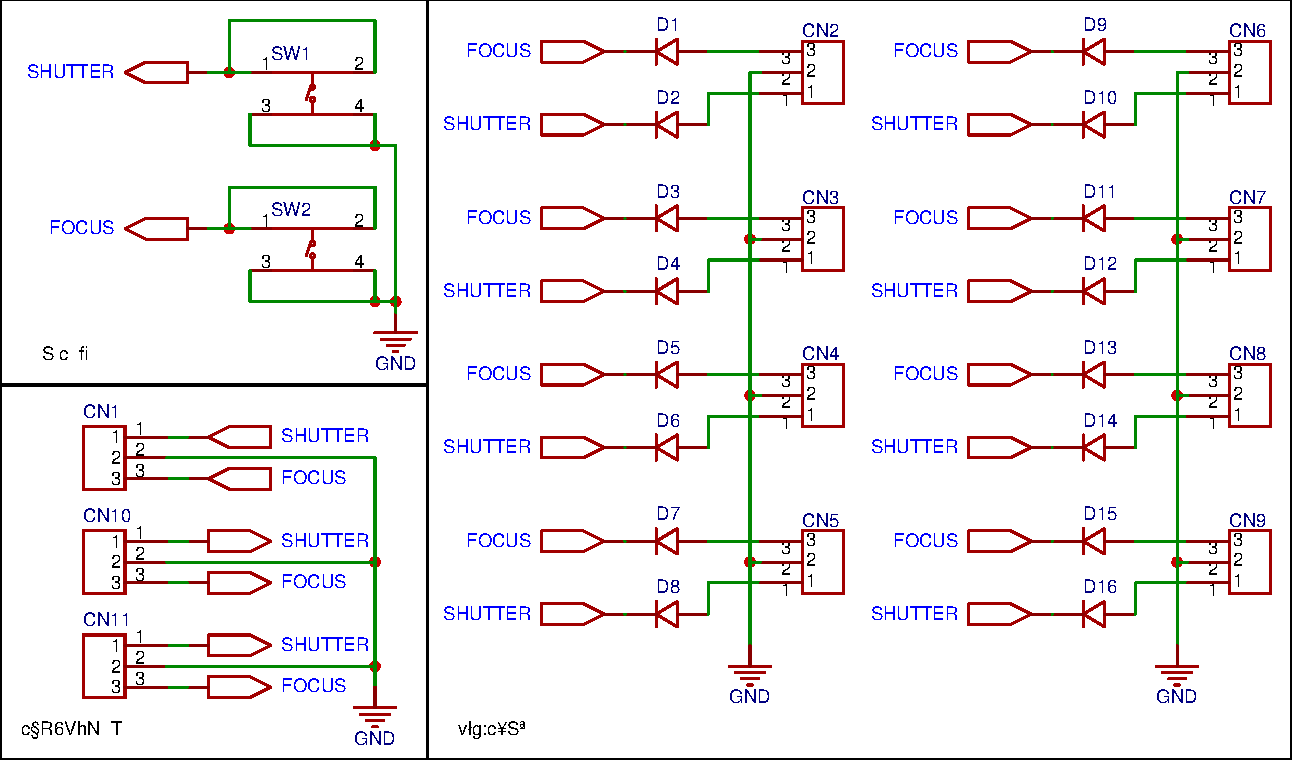
\includegraphics[width=\textwidth]{figures/passive_sync_schematic}
    \caption{被动控制器的电路原理图}
    \label{fig:passive_sync_schematic}
\end{figure}
\begin{figure}
    \centering
    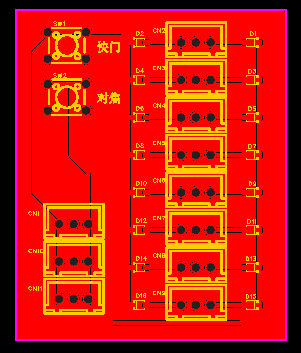
\includegraphics{figures/passive_sync_pcb}
    \caption[被动控制器的PCB布局]{被动控制器的PCB布局。1:1尺寸比例}
    \label{fig:passive_sync_pcb}
\end{figure}
每个被动控制器的电路原理图如图\ref{fig:passive_sync_schematic}所示,
该电路实现为一块简单的单面布线板,其布局如图\ref{fig:passive_sync_pcb}所示。
右侧8个XH2.54-3P插座用于连接相机,它们分别经过1N4148WS二极管后连接到合并的控制线上。
左侧3个XH2.54-3P插座则用于控制器之间的连接,不经过二极管。
左上角两颗$6\times 6$mm的轻触开关用于实现控制线与地线的短接,以便于触发对应的控制功能。


\chapter{主动同步控制器实现细节}
\label{app:active_sync}

\begin{figure}[p]
    \centering
    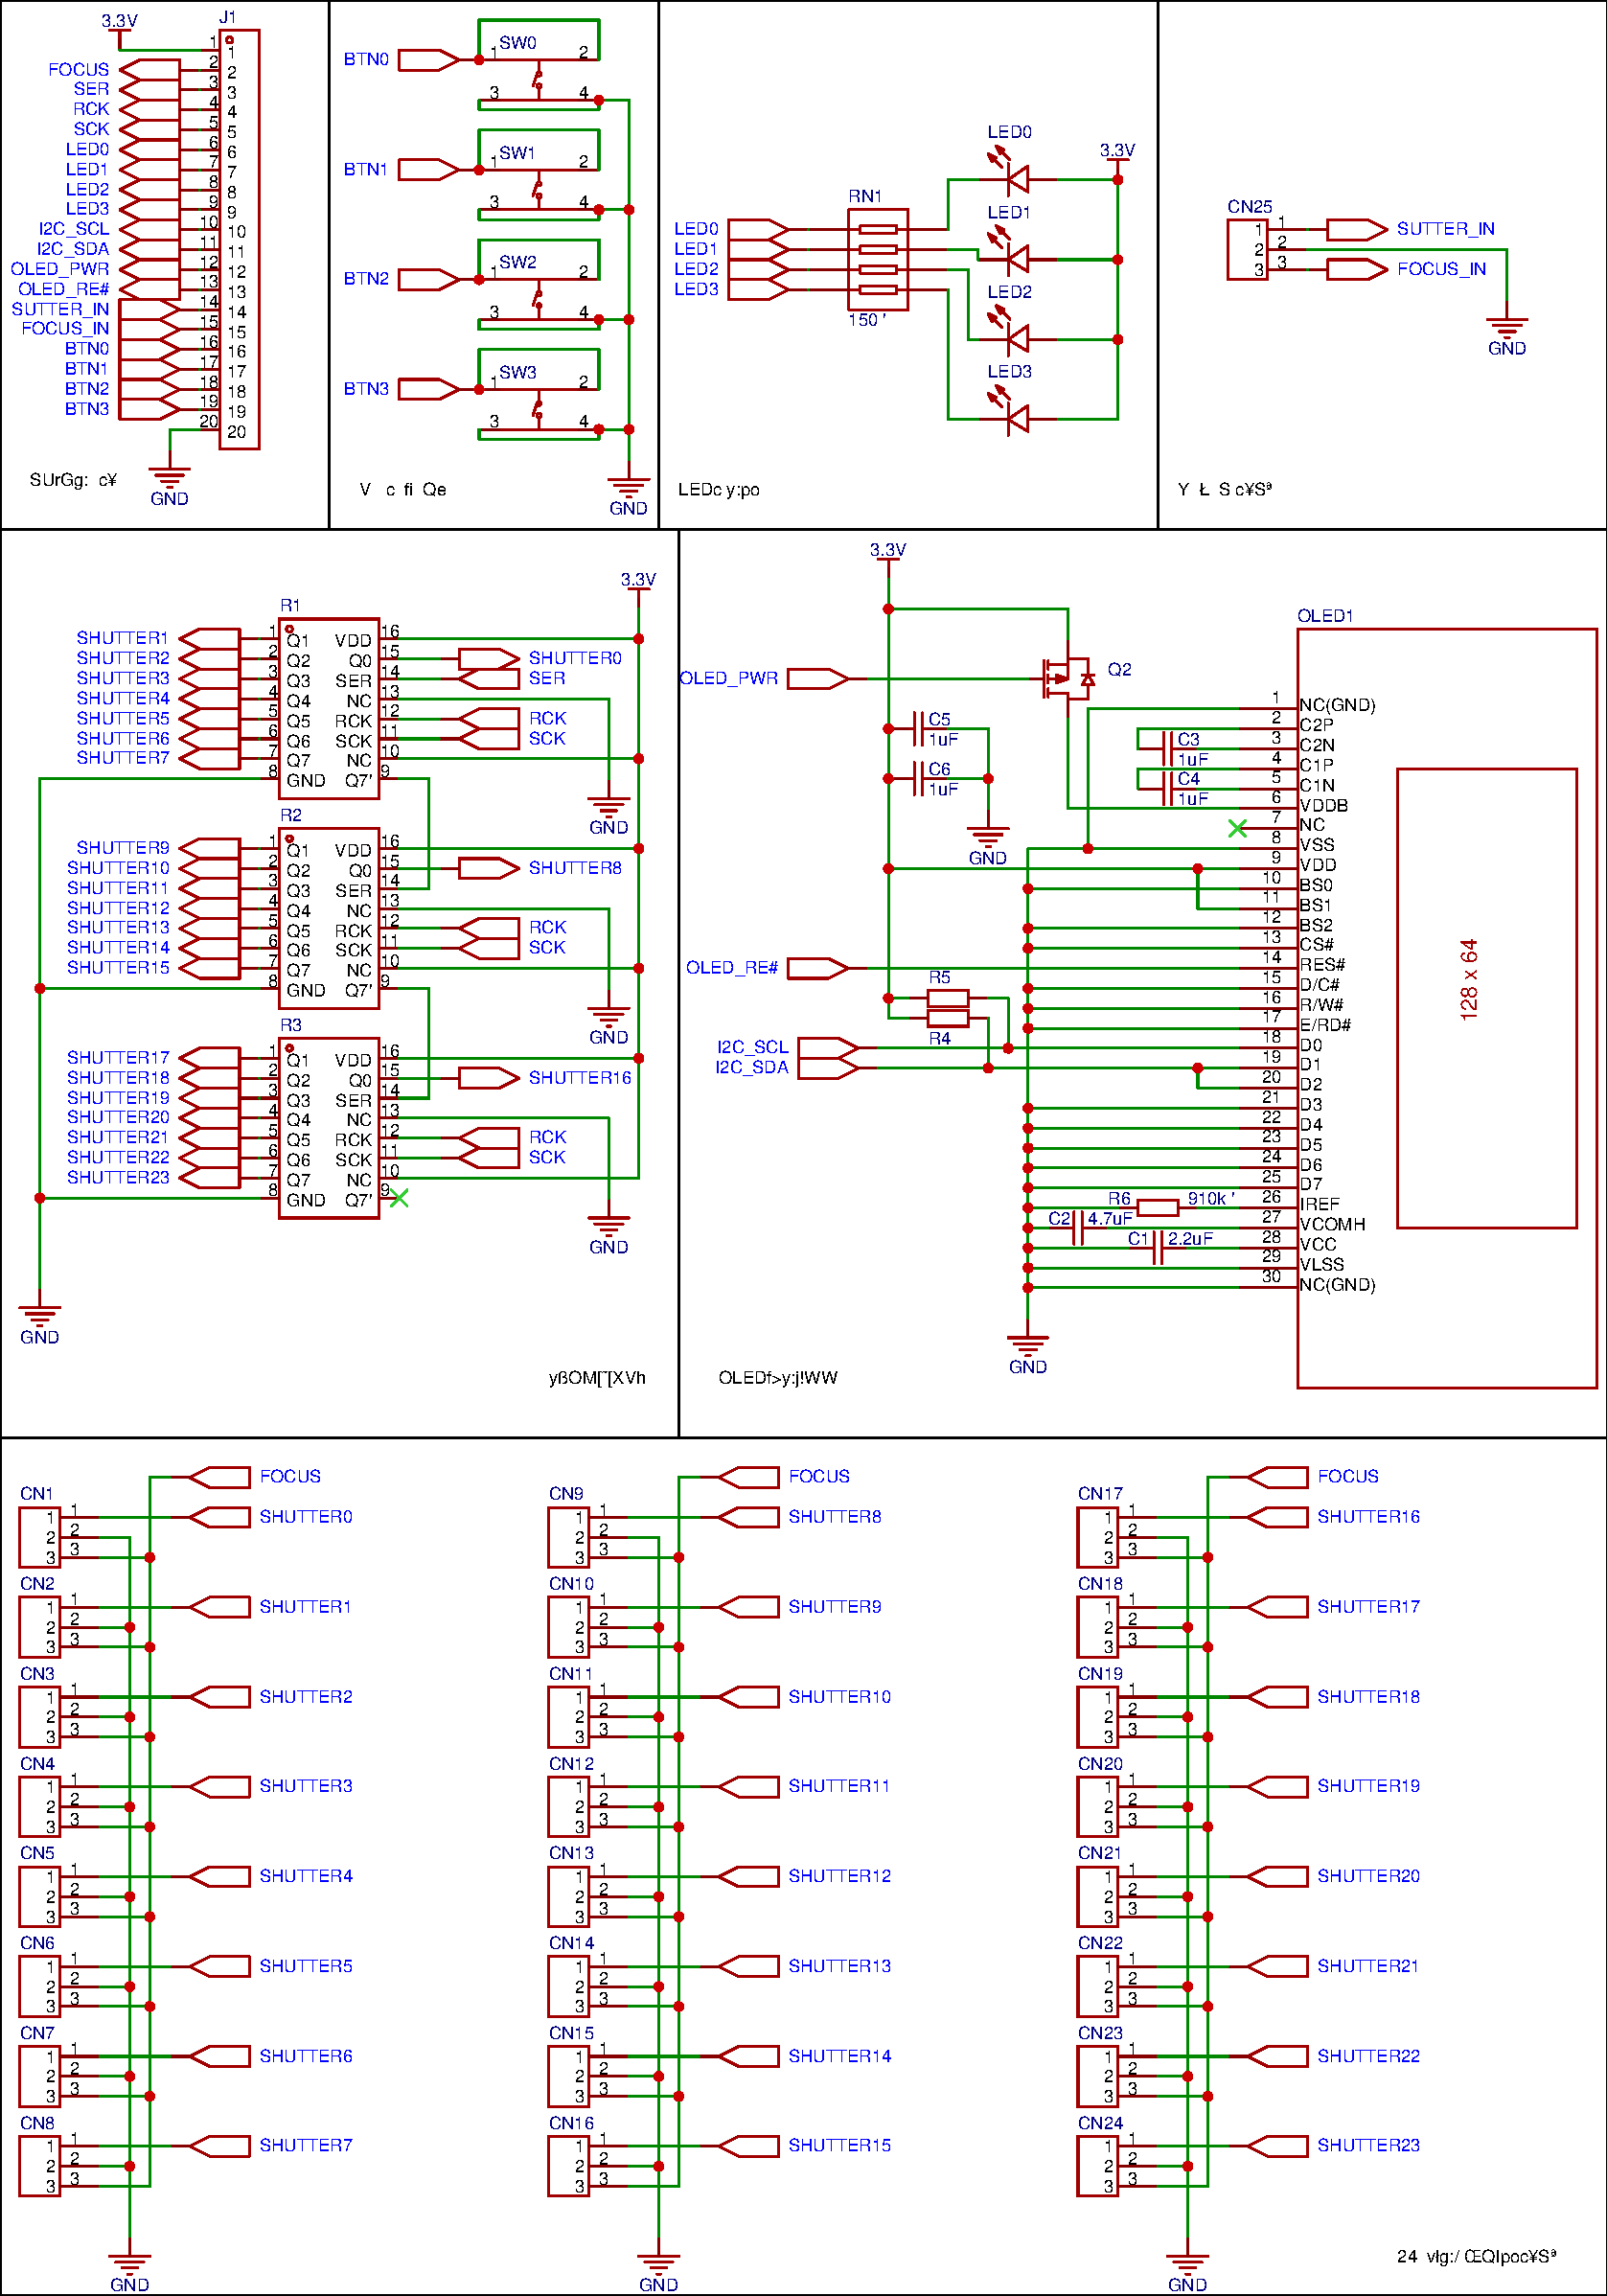
\includegraphics[width=\textwidth]{figures/active_sync_schematic}
    \caption{主动控制器的电路原理图}
    \label{fig:active_sync_schematic}
\end{figure}
\begin{figure}
    \centering
    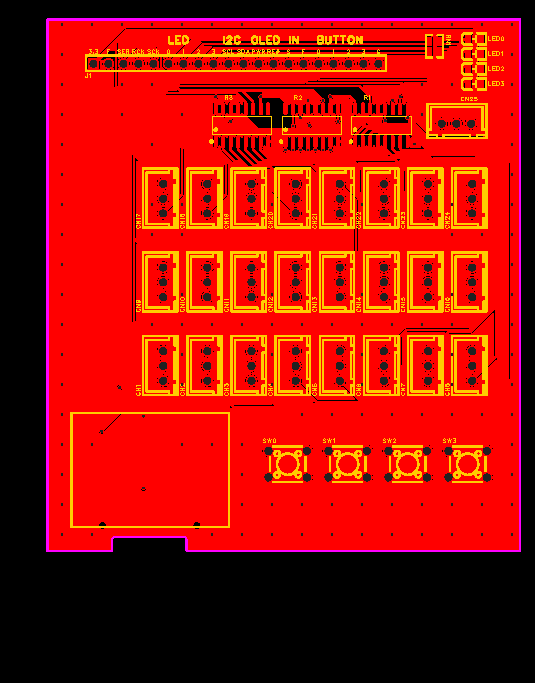
\includegraphics[page=1]{figures/active_sync_pcb}
    \includegraphics[page=2]{figures/active_sync_pcb}
    \caption[主动控制器的PCB布局]{主动控制器的PCB布局。1:1尺寸比例}
    \label{fig:active_sync_pcb}
\end{figure}
\paragraph{硬件}
主动同步装置的控制器实现为三块相互独立的电路板,
电路板之间使用20P的排针和排母连接。
其中包括一块市面上购买的STM32最小系统板,一块定制的布置了所有所需IO外设的IO板,
以及一块定制的用于连接两者的连接板。
之所以设计独立的一块连接版,是为了在不重新制作现有IO板的情况下,更改其与单片机的连接方式,也便于今后在同一片最小系统板上连接更多外设。
其中IO板的电路原理图如图\ref{fig:active_sync_schematic}所示。
该电路实现为一块双面布线的PCB,其布局如图\ref{fig:active_sync_pcb}所示。

其中OLED显示器使用SSD1306芯片,分辨率为$128\times 64$,显示区域尺寸0.96英寸。
STM32单片机通过硬件I2C接口与OLED显示器通信。
所采用的移位寄存器芯片为富满FM的74HC595D,其输出引脚的驱动方式为开漏输出,这可以避免不同独立供电的设备间电压不匹配造成的潜在问题。
在该方案中,每个相机的接口不再需要二极管,而可以直接连接到移位寄存器的输出引脚上。
其接口依然使用的是和被动同步控制器相同的XH2.54-3P插座,因此与相机和连接线可以共用。
OLED显示模块的电路设计则直接参考了相关数据手册中的参考电路。
但由于本方案中VDDB和VDD的供电来自同一条线路,因此省略了一个场效应管。

\clearpage
\paragraph{软件}
\begin{figure}
\centering
\begin{tikzpicture}[
    node distance=.2cm,
    every node/.style={outer sep=0pt,draw,anchor=south west},
    every fit/.style={inner sep=0pt},
    placeholder/.style={draw=none},
    fill_text/.style={draw=none,anchor=center},
    ]
    \node (event_p) [placeholder] {\vphantom{事件循环}};
    \node (btn) [above=of event_p.north west,anchor=south west] {按键检测};
    \node (ui_mgr_p) [placeholder,right=of btn] {\vphantom{图形界面管理}};
    \node (menu) [above=of ui_mgr_p.north west,anchor=south west] {菜单};
    \node (delay_overview) [right=of menu] {延迟概览};
    \node (num) [right=of delay_overview] {数值设置};
    \node (trigger) [right=of num] {触发};
    \node (about) [right=of trigger] {关于};
    \node (toast) [right=of about] {消息框};


    \node (oled_p) [above=of menu.north west,anchor=south west,placeholder] {\vphantom{OLED显示控制}};

    \node (oled_fit) [fit=(oled_p)(oled_p-|toast.east)] {};
    \node [fill_text] at (oled_fit) {OLED显示控制};

    \node (ui_mgr_fit) [fit=(ui_mgr_p)(ui_mgr_p-|toast.east)] {};
    \node [fill_text] at (ui_mgr_fit) {图形界面管理};

    \node (event_fit) [fit=(event_p)(event_p-|toast.east)] {};
    \node [fill_text] at (event_fit) {事件循环};

    \draw [->] (btn)++(0,2cm) -- node [left,draw=none] {中断} (btn);
\end{tikzpicture}
\caption{主动同步控制器的软件架构}
\label{fig:active_sync_software_arch}
\end{figure}
在主动同步控制器的单片机中运行的固件架构如图\ref{fig:active_sync_software_arch}所示。
该程序使用C++编写,不运行于操作系统之上。
该程序最外层为事件循环,它负责获取按键输入,将输入事件传递给图形界面模块,
并适时地休眠以节省电量。
按键检测模块负责响应按钮产生的硬件中断,产生输入事件,并过滤由于机械抖动产生的干扰信号。
图形界面管理模块负责维护当前打开的图形界面栈,处理打开新页面,和返回上一页面的请求,并将输入事件传递给栈顶的图形界面。
运行在图形界面管理模块之上的是各种具体的界面,它们负责真正处理输入事件,执行相应逻辑,并调用OLED显示控制模块来更新显示内容。
其中,菜单模块在构造时接收一个带有回调函数的菜单项列表,用于支持各种不同的菜单;
数值设置模块则使用traits模式,通过模板参数以支持不同的数值类型、数值范围和数值存储位置等,可支持触发延迟、休眠时间、屏幕对比度等诸多数值设置需求。
OLED显示控制模块负责调用单片机的硬件I2C接口与OLED显示器通信,
并封装了一些常用的绘图函数,如文本渲染等。

在菜单的导航中,从左到右四个按钮的功能分别定义为:上一项,确认,下一项,返回;
在数值设置界面,这些按钮则分别为:减小,切换开启/关闭,增大,确认。

值得一提的是,在延迟设置的界面,用户可设置的最小分辨率为0.1毫秒,且最大范围为5秒,共50000个不同的设置值。
但本装置只有4个按钮,为了能快速设置到需要的值,本文设计了一种特殊的交互方式。
当用户按住增大按钮时,数值将不断增大,其增大的速度分为三个阶段:
在按钮按下时数值增大0.1毫秒,0.5秒内不再增大;
在0.5秒到2秒内,数值每0.1秒增大0.1毫秒;
在2秒后,数值与按住的时间呈二次函数关系:若当前按钮按住的时间为$2+t$秒,最大设定值为$m=5$秒,设定数值的增量在之前线性增加的基础上,再额外增加$m(t/10)^2$,
即在10秒内数值增量相当于整个设置范围。
如此即可兼顾定位的准确性和大范围移动的便利性。
得益于本方案使用的traits设计模型,其他数值设置也能复用这一交互方式,只需在traits中定义好数值的范围,增量大小等即可。
在未来也可借助滚动编码器等额外硬件以提供更好的用户体验。

\chapter{照片整理工具实现细节}
\label{app:pick_photo_impl}

第\ref{sec:photo_process}节中提到,本方案中包括了一款照片整理工具,
并已经介绍了其主要功能。
本附录将介绍该工具的具体实现细节。

本工具是一个简单的B/S架构的Web应用,其后端使用Python基于aiohttp框架实现,
前端使用Vue.js框架实现。

后端的主要工作为:
\begin{enumerate}
\item 收集需要整理的照片列表,提取其元数据;
\item 加载和保存已整理好的照片分组和快门匹配数据,以及相机间时间戳的偏移量。
\end{enumerate}
为实现这些功能,后端在启动时接收一个文件夹路径作为参数,
需要整理的照片包括该文件夹下的所有CR3文件,
数据则直接保存到相同文件夹下的json格式文件中,以便对接后续处理步骤的程序。
本方案中使用的相机并不能自行校准时间戳,在一个月的时间内,之前手动校准的时间戳之间就会产生数分钟的偏差。
为避免反复手动调整相机时钟设置,本工具支持在显示时自动添加偏移。
相机间时间戳的偏移量存储于单独的文件中,用户可以复用之前拍摄时的数据,以避免从头开始校准,降低校准的难度。
在提取CR3格式的照片元数据时,本工具根据网上公开的CR3格式反向工程文档\footnote{\url{https://github.com/lclevy/canon_cr3}},自行实现了格式解析器。
该解析器经测试在磁盘IO完全命中操作系统缓存的前提下,比开源的ExifTool\footnote{\url{https://exiftool.org/}}快约260倍,且不依赖于外部程序,使用更加简单。
后端总共为前端提供如下5个HTTP RESTful API:
\begin{enumerate}
\item GET /photos:获取照片列表,及其元数据;
\item GET /photos/\{id\}/thumbnail:获取指定照片的缩略图;
\item GET /photos/\{id\}/jpg:获取指定照片中内嵌的JPG格式全分辨率预览图;
\item GET /grouping:获取先前保存的已整理好的照片分组等;
\item POST /grouping:保存已整理好的照片分组等;
\end{enumerate}

前端所实现的功能参见图\ref{fig:pick_photo},
这里补充一些实现的细节。
界面下方主体区域可纵向和横向滚动,画布中的照片可根据其所属相机和拍摄时间精确定位,这是使用Vue的模板生成SVG元素实现的。
在界面加载时若没有可用的分组数据,且在计算相机时间戳偏移后连续1分钟内没有任何照片,则将长空隙前后部分自动分割为不同分组。
不同分组间的时间间隔将不会在界面中体现,以避免过长的横向滚动条。

关于“识别捕获”按钮所使用的贪婪算法:
即使经过了时间戳的对齐,同一次快门捕获的照片仍然会因为未知原因时间戳稍有不同。
且由于接触不良或相机响应速度不足等原因,某些相机偶尔会漏触发某次快门,因此无法仅根据拍摄照片的序号判断是否是同一次捕获。
为在存在噪音的情况下尽可能准确地识别出同一次捕获的照片,本工具使用了如下算法:
\begin{enumerate}
\item 对每张照片,在每台除自己外的相机中各挑选一张时间戳最靠近自己的照片作为潜在的匹配;
\item 假设所有照片均为独立的捕获;
\item 对所有潜在匹配排序,时间戳误差从低到高。
\item 遍历所有潜在匹配,若匹配中的两张照片不属于同一次捕获,且两者各自的捕获中包含的相机没有交集(同一台相机不可能在同一次捕获中输出两张照片),则合并该两个捕获,认为其是同一次捕获。
\end{enumerate}
如此便能得到一个捕获的集合,其中每个捕获中的照片的时间戳尽可能接近,且没有重复的相机。
\begin{figure}
\includegraphics[width=\textwidth,trim={10 10 10 120},clip]{figures/pick_photo_capture}
\caption{“捕获”状态照片整理工具UI截图}
\label{fig:pick_photo_capture}
\end{figure}
图\ref{fig:pick_photo_capture}展示了选中“捕获”单选按钮时,界面上显示捕获识别的结果的截图。


\backmatter
\chapter{攻读硕士学位期间取得的研究成果}

一、已发表(包括已接受待发表)的论文,以及已投稿、或已成文打算投稿、或拟成文投稿的论文情况:

\noindent\begin{tabularx}{\textwidth}{| p{0.5cm} | X | p{1.8cm} | p{1.7cm} | p{1.8cm} | p{1.8cm} |}
\hline
\textbf{序号} & \textbf{发表或投稿刊物/会议名称} & \textbf{作者} & \textbf{发表年份} & \textbf{与学位论文哪一部分相关} & \textbf{被索引收录情况} \\
\hline
 & & & & & \\
\hline
\end{tabularx}

\vskip 0.5cm

二、与学位内容相关的其它成果(包括专利、著作、获奖项目等):

\hideinblind{
\chapter{致谢}

研究生三年的时光转瞬即逝。
这三年来,我虽有遗憾,但更多的是收获和成长,并度过了一段充实的学生生涯。
相比三年前,我在知识的深度和广度上均有提升,
我深知,这是在导师的指导和同学,以及其他一些人的帮助下才能实现的,我向他们表示感谢。
我首先要感谢我的导师杜卿老师,她温柔耐心、循循善诱,她也对本文的写作给予了很多的建议。
我还要感谢谭明奎教授,他在我的研究方向尚不明朗时为我提供了很多建议和帮助。
谭教授也为我们创造了舒适的实验室环境,并提供了高性能的机器学习计算资源。
特别要感谢CVTE和王乃洲博士,本文的工作也是华南理工大学与CVTE合作项目的成果,
CVTE为本文的所有实验提供了经济支持。
感谢嘉立创公司提供的免费PCB打样服务,让我这个软件专业的学生也能有机会实现自己定制的硬件。
同时,我要感谢我的同学们,与他们相处我感到很快乐,他们也给予了我很多的帮助。
最后,感谢强盛的祖国,和平的时代,富饶的社会,以及无数为之而奋斗的先辈们,所有人的努力造就了今天令人安心的科研环境。
}% end hideinblind



\end{document}
